%/**
% * LaTeX thesis template (main file)
% * @author : Alexander willner <alex@willner.ws>
% * @url    : http://github.com/thesis
% */

% include config ---------------------------------------------------------------
\RequirePackage{pdf14}                 % PDF/A2-b compatibility
%\PassOptionsToPackage{demo}{graphicx} % for faster drafts
% document configuration -------------------------------------------------------
\documentclass[
        pagesize,               % put paper size information into document
        a4paper,                % use a5paper for ISO A5; use a4paper for ISO A4
        pdftex,                 % PDF output
        fontsize=12pt,          % font size
        headsepline,            % use headinclude also! (see M. Kohm)
        footsepline,            % use footinclude also! (see M. Kohm)
        headinclude,            % count head to text body (not to margin)
        footinclude,            % count foot to text body (not to margin)
        BCOR8mm,                % set extra margin for book fixation
        headsepline,            % line on the top
        openany,                % allows chapters to occur on left hand pages
        titlepage,              % show a title page
        draft=false,            % show under-/overfull boxes
        DIV=calc                % calculate a nice type area
        %ngerman,                % German language support
        %numbers=noendperiod     % no number at the end (German DUDEN)
]{scrbook}
% ------------------------------------------------------------------------------

% lang config ------------------------------------------------------------------
%\usepackage{CJKutf8}                         % Japanese language support
%\usepackage[ngerman]{babel}                  % German language support
%\usepackage{bibgerm}                         % German bibliography support
%\usepackage[babel,german=quotes]{csquotes}   % German language support
% lang config ------------------------------------------------------------------

% basic config -----------------------------------------------------------------
\usepackage{tocloft}                          % Tweaks for large ToCs
\cftsetpnumwidth{2em}

\makeatletter
\providecommand{\IfPackageLoaded}[2]{\@ifpackageloaded{#1}{#2}{}}
\providecommand{\IfPackageNotLoaded}[2]{\@ifpackageloaded{#1}{}{#2}}
\providecommand{\IfElsePackageLoaded}[3]{\@ifpackageloaded{#1}{#2}{#3}}
\makeatother

\IfPackageNotLoaded{CJKutf8}{\usepackage[utf8x]{inputenc}} % File encoding: Normal UTF8
\usepackage{cmap}                     % Support copy and search
\usepackage[tracking=true,            % Fonts: hyphenatable letterspacing
expansion=true,                       % Fonts: better grey value
protrusion=true]{microtype}           % Fonts: margin kerning
\usepackage[T1]{fontenc}              % Font encoding: T1
\usepackage{textcomp}                 % For the Euro sign
\usepackage{booktabs}                 % Nice tables
\usepackage{listings}                 % Nice listings
\usepackage{url}                      % Create URLs in the document
\usepackage{color}                    % To use and define colors
\definecolor{LinkColor}{rgb}          % Link color
{0.31,0.46,.64}                       %
\definecolor{MarginColor}{rgb}        % Margin color
{0.31,0.46,.64}                       %
\usepackage[pdftex]{graphicx}         % Include images in PDFs
\usepackage[pdftex,                   % Hyperlinks in PDFs
raiselinks=true,			          % calculate real height of the link
breaklinks,                           % break links
backref=page,                         % backlinks in bibliography (section, slide, page, none)
pagebackref=true,                     % backlinks in bibliography
hyperindex=true,                      % backlinkex index
linktocpage=true,                     % ToC links pages
bookmarks=true,                       % Bookmarks for PDF viewers
bookmarksopen=true,                   % Open bookmarks
bookmarksopenlevel=1,                 % How many levels to open
bookmarksnumbered=true,               % Numbers in the bookmarks
bookmarkstype=toc,                    % Type of bookmark
plainpages=false,                     % Anchors even on plain pages?
pageanchor=true,                      % Pages are linkable
pdfstartview=FitH,                    % Open document with Fit Width
pdfpagelabels=true,                   % set PDF page labels
pdfpagemode=UseOutlines,              % Show bookmarks in viewer
colorlinks,                           % Show colored links
linkcolor=LinkColor,                  % Link color
urlcolor=LinkColor,                   % URL color
anchorcolor=LinkColor,                % Anchor color
citecolor=LinkColor,                  % Cite color
menucolor=LinkColor,                  % Menu color
hypertexnames=true                    % Whatever ;)
]{hyperref}                           % Use hyperlinks
\renewcommand*{\backref}[1]{[cited at page #1]}% Show formatted backlinks
\usepackage{marginnote}               % Non floating margin notes
\usepackage[caption=false]{subfig}    % Many figures in one environment
\usepackage{stfloats}                 % Makes LaTeX honour ‘[b]’ placement
\usepackage{amssymb}                  % Springer Verlag
\usepackage{amsmath}                  % For eqref
\usepackage{acronym}                  % For acronyms
\usepackage{paralist}                 % For inline lists
\usepackage{fixltx2e}                 % Provides fixes for LaTeX
\usepackage{fix-cm}                   % Provides fixes for LaTeX
\usepackage{rotating}                 % e.g. for the special side margin notes
\usepackage{lipsum}                   % To add some dummy text
\usepackage{xspace}                   % Fixing some spacing issues
\usepackage{ellipsis}                 % Puts space around ellipses
\usepackage{ragged2e}                 % New commands/env. for setting ragged text
\usepackage[bf]{caption}[2008/08/24]  % Bold caption (better contrast)
\newcommand{\etc}{etc.\@\xspace}      % Fixing some spacing issues
\lstset{columns=fullflexible}         % Listings in multicolumn mode

\hyphenation{op-tical net-works semi-conduc-tor con-cept}

\renewcommand{\figurename}{Fig.}
\renewcommand{\tablename}{Tab.}
\newcommand{\sectionname}{Sec.}
\newcommand{\equationname}{Eq.}

\makeindex

\setcounter{tocdepth}{3}
\newcommand{\mykeywords}[1]{\par\addvspace\baselineskip
\keywordname\enspace\ignorespaces#1}
\makeatletter
\providecommand*{\toclevel@title}{99}
\providecommand*{\toclevel@author}{99}

\setlength{\marginparwidth}{0.7in}
\newcommand\note[1]{%
  \marginnote{%
    \scriptsize%
    \raggedright%
    \hspace{0pt}%
    \color{MarginColor}%
    %\begin{turn}{270}\emph{#1}\end{turn}
    \emph{#1}
  }
}

\newcommand{\annot}[2][]{%
  \pdfannot width \linewidth height 2\baselineskip depth 0pt{%
    /Subtype/Text%
    /Open false
    /Name /Comment%
    /CA .4%
    /C [.3 .6 .9]%
    /T (\pdfescapestring{#1})%
    /Contents(\pdfescapestring{\detokenize{#2}})%
  }
}
          % Default config
% basic config -----------------------------------------------------------------

% local config -----------------------------------------------------------------
\usepackage{scrhack}                          % Fix some scrbook issues
\usepackage[numbers,square,longnamesfirst]{natbib}  % Bibliography: style
\definecolor{LinkColor}{rgb}{0,0,0}           % Link color
\definecolor{MarginColor}{rgb}{.29,.03,.06}   % Link color
\usepackage[printonlyused,withpage]{acronym}  % Acronyms
\usepackage[Sonny]{fncychap}                  % Nice chapter header
\usepackage{wallpaper}                        % To show an icon on the first page
\usepackage{minitoc}                          % ToC for chapters
\dominitoc[n]                                 % No caption for mini ToCs
\addtokomafont{sectioning}{\rmfamily}         % Serifs in headings
\ChNameVar{\Large\rmfamily}                   % Fancy chapter with serifs
\ChTitleVar{\Large\rmfamily}                  % Fancy chapter with serifs
\renewcommand*{\acsfont}[1]{{\rmfamily{#1}}}
\renewcommand{\lstlistlistingname}{List of Algorithms}
\renewcommand{\lstlistingname}{Algorithm}
\usepackage{mathptmx}                % Nicer fonts (for all) - times
%\usepackage[clearempty]{titlesec}    % Suppress header and footer for empty pages
\usepackage{makeidx}                 % Make an index
\makeindex                           % Make an index
\newlength\cornerXoffset
\newlength\cornerYoffset
\setlength\cornerXoffset{0cm}        % X
\setlength\cornerYoffset{2cm}        % Y
\newcommand\ThisLROffsetCornerWallPaper[2]{%
  \AddToShipoutPicture*{%
    \AtPageLowerLeft{%
      \parbox[b]{\paperwidth-\cornerXoffset}{%
        \hfill \includegraphics[width=#1\paperwidth,height=#1\paperheight,%
        keepaspectratio]{#2}%
        \vspace{\cornerYoffset}\null
      }
    }
  }
}

\setcounter{secnumdepth}{4}
\setcounter{tocdepth}{4}
% ------------------------------------------------------------------------------


% fix for old tex installations ------------------------------------------------
% ------------------------------------------------------------------------------


% page layout ------------------------------------------------------------------
\usepackage{geometry}
\geometry{a4paper, bottom=4cm}
\renewcommand{\topfraction}{0.9}
\renewcommand{\bottomfraction}{0.9}
\renewcommand{\textfraction}{0.07}         % allow minimal text w. figs
\renewcommand{\floatpagefraction}{0.7}     % require fuller float pages
\renewcommand{\dblfloatpagefraction}{0.7}  % require fuller float pages
\renewcommand{\dbltopfraction}{0.9}        % fit big float above 2-col. text
\renewcommand{\textfloatsep}{5mm}
\setcounter{topnumber}{2}
\setcounter{bottomnumber}{2}
\setcounter{totalnumber}{4}                % 2 may work better
\setcounter{dbltopnumber}{2}               % for 2-column pages

%\ChNameVar{\vspace*{-1in}\Large\sf}
%\ChNumVar{\vspace*{-1in}\Huge}
%\ChTitleVar{\vspace*{-1in}\Large\sf}
%\ChRuleWidth{0.5pt}
%\ChNameUpperCase

%\makeatletter
%\def\@makeschapterhead#1{%
%  \vspace*{0\p@}
%  {\parindent \z@ \raggedright
%    \normalfont
%    \interlinepenalty\@M
%    \DOTIS{#1}
%    \vskip 0\p@
%  }}
%\makeatother
% ------------------------------------------------------------------------------

% hyperlinks (almost last package) --------------------------------------------
\usepackage{hyperxmp}                 % Semantic meta data (RDF/XMP)
\usepackage[pdftex,                   % Hyperlinks in PDFs
raiselinks=true,			          % calculate real height of the link
breaklinks,                           % break links
%backref=page,                         % backlinks in bibliography (section, slide, page, none)
%pagebackref=true,                     % backlinks in bibliography
hyperindex=true,                      % backlinkex index
linktocpage=true,                     % ToC links pages
bookmarks=true,                       % Bookmarks for PDF viewers
bookmarksopen=true,                   % Open bookmarks
bookmarksopenlevel=2,                 % How many levels to open
bookmarksnumbered=true,               % Numbers in the bookmarks
bookmarkstype=toc,                    % Type of bookmark
plainpages=false,                     % Anchors even on plain pages?
pageanchor=true,                      % Pages are linkable
pdfstartview=FitH,                    % Open document with Fit Width
pdfpagelabels=true,                   % set PDF page labels
pdfpagemode=UseOutlines,              % Show bookmarks in viewer
colorlinks,                           % Show colored links
linkcolor=LinkColor,                  % Link color
urlcolor=LinkColor,                   % URL color
anchorcolor=LinkColor,                % Anchor color
citecolor=LinkColor,                  % Cite color
menucolor=LinkColor,                  % Menu color
hypertexnames=true                    % Whatever ;)
]{hyperref}                           % Use hyperlinks
%\renewcommand*{\backref}[1]{[cited at page #1]} % Show formatted backlinks
\usepackage{bookmark}                         % Manually add PDF bookmarks
% ------------------------------------------------------------------------------

% glossary (last package) ----------------------------------------------------
\usepackage[xindy,nonumberlist,toc]{glossaries}
\input{\metaFilename.glos.tex}
\renewcommand*{\glossaryname}{Glossary}
\setglossarystyle{altlist}
\renewcommand*{\glsgroupskip}{}
%fixme: the glossary moves the minitocs to the wrong chapters
\renewcommand*{\gls}[1]{{#1}}
%\makeglossaries
% ------------------------------------------------------------------------------

% meta data --------------------------------------------------------------------
\input{\metaFilename.meta}
%%% Only for koma script
%\subject{\metaSubject}
%\title{\metaTitle}
%\author{\metaAuthor}
%\date{\metaDate}
%\dedication{\metaDedication}

\hypersetup{
      pdfauthor={\metaAuthorShort~<\metaAuthorMail>},
      pdfsubject={\metaSubject},
      pdftitle={\metaTitle},
      pdfkeywords={\metaKeywords},
      pdfcreator={LaTeX},
      pdfproducer={LaTeX},
}

% ------------------------------------------------------------------------------
     % inlcude general configuration
%\DeclareAcronym{PLC}{short={PLC}, long={Programmable Logic Controller}}
%\DeclareAcronym{Swoogle}{short={Swoogle}, long={}, cite={ding2004swoogle}, long-post={\acfootnote{\url{http://swoogle.umbc.edu}}}}
%\DeclareAcronym{}{short={}, long={}, short-indefinite={an},  long-indefinite={an}, cite={}, long-post={\acfootnote{\url{}}}, class=exclude}
%\DeclareAcronym{}{short={}, long={}}
\DeclareAcronym{ABAC}{short={ABAC}, long={Attributed Based Access Control}, cite={li2002design,Yuan2005}}
\DeclareAcronym{DBpedia}{short={DBpedia}, long={DBpedia}, cite={Auer2007}, long-post={\acfootnote{\url{http://dbpedia.org}}}, class=exclude}
       % inlcude acronyms
\DeclareUnicodeCharacter{0301}{}       % fixing an UTF-8 encoding issue
%\usepackage[norefs,nocites]{refcheck} % useful, but not working with cref
%\usepackage[doublespacing]{setspace}  % useful for reviewing a printout
%\PassOptionsToPackage{cmyk}{xcolor}   % PDF/A compatibility, skipped
%\usepackage[a-2b]{pdfx}               % PDF/A compatibility, skipped
\newcommand{\isFinal}{true}            % Modify e.g. the title page
% ------------------------------------------------------------------------------


% include only required files for faster building ------------------------------
%\includeonly{src/03_requirements,src/06_implementation}
% ------------------------------------------------------------------------------


% begin thesis -----------------------------------------------------------------
\begin{document}
    \frontmatter
    \pagestyle{empty}
    \pagenumbering{alph}
    \pdfbookmark{Title}{title}
\begin{titlepage}
\newgeometry{left=35mm, right=35mm, top=35mm, bottom=35mm}


\begin{center}
\vspace*{2cm}
\LARGE{\metaTitleLayouted}\\
\normalsize

\vspace*{2cm}
\metaSubmitted%
\\
\metaAuthor, \metaDegree~\\
\metaBirthplace%
\\

\vspace*{2cm}
\metaFaculty%
\\
\metaUniversity%
\\
\metaWhy%
\\
\vspace*{0,5cm}
\metaType%
\\
-~{\metaTypeShort}~-% chktex: 8
\\
\vspace*{0,5cm}

\ifthenelse{\equal{\isFinal}{true}}{
\metaHowFinal%
}{
\metaHowNonFinal%
}
\end{center}

\ifthenelse{\equal{\isFinal}{true}}{

\vspace*{2cm}
\metaBoard:\\
\vspace*{.3cm}\\
\begin{tabular}{@{\hspace{1.5em}}ll}
\metaChair: & \metaChairName~(\metaChairUniversity) \\
\metaReviewer: & \metaFirstReviewerName~(\metaFirstReviewerUniversity) \\
\metaReviewer: & \metaSecondReviewerName~(\metaSecondReviewerUniversity)\\
\metaReviewer: & \metaThirdReviewerName~(\metaThirdReviewerUniversity)\\
\end{tabular}

\vspace*{1,9cm}
\metaDateExam%
\vspace*{0,9cm}

}{
\vspace*{6cm}
}

\begin{center}
\metaNumber\newline
\end{center}


\ThisLROffsetCornerWallPaper{.2}{resources/images/logo}   % logo in the corner

\restoregeometry%
\end{titlepage}

    \cleardoublepage\vspace*{100mm}
\begin{minipage}{109.5mm}
\section*{Affidavit}
I hereby declare that the following thesis ``\metaTitle'' has been
written only by the undersigned and without any assistance from third
parties.\\

Furthermore, I confirm that no sources have been used in the preparation
of this thesis other than those indicated in the thesis itself.\\[2cm]
\metaCity,
\metaDate%
\end{minipage}

    \cleardoublepage\pdfbookmark{Dedication}{dedication}
\begin{center}
\LARGE{\metaDedication}
\end{center}

    \cleardoublepage

    \pagestyle{scrheadings}
    \lohead[]{}
    \pagenumbering{roman}
    \setcounter{page}{1}
    \pdfbookmark{Acknowledgments}{acknowledgments}
\chapter*{Acknowledgments}

\todomid{thank your supervisors}

\todomid{thank your colleagues}

\todomid{thank your family and friends}

\vspace{0.5in}
\begin{flushright}
  \metaCity, February 12, 2016%\today%
\end{flushright}
\cleardoublepage{}
    \pdfbookmark{Abstract}{abstract}
\chapter*{Abstract}

{\setlength{\parindent}{-.1cm}%
\sidenote{Research Area:\\Foo Bar}%
\todomid{write about the research area}

\sidenote{Application Area:\\Bar Foo}
\todomid{write about the application area}

\sidenote{Research Issue:\\Foo Fooli}
\todomid{write about the research issue}

\sidenote{Own Approach:\\Bar Barli}
\todomid{write about the own approach}

\sidenote{Scientific Contributions}
\todomid{write about the scientific contributions}

\sidenote{Validation \& Outlook}
\todomid{write about the validation and outlook}

\cleardoublepage
\begin{otherlanguage}{ngerman}
\pdfbookmark{Zusammenfassung}{Zusammenfassung}
\chapter*{Zusammenfassung}%

\sidenote{For\-schungs\-be\-reich:\\Foo Bar}%
\todomid{write}

\sidenote{Ein\-grenz\-ung:\\Bar Foo}
\todomid{write}

\sidenote{Pro\-blem\-stel\-lung:\\Foo Fooli}
\todomid{write}

\sidenote{Eigener Ansatz:\\Bar Barli}
\todomid{write}

\sidenote{Wis\-sen\-schaft\-lich\-er Bei\-trag}
\todomid{write}

\sidenote{Va\-li\-die\-rung \& Aus\-blick}
\todomid{write}

\end{otherlanguage}

}
\cleardoublepage
\cleardoublepage

    \phantomsection
    % Change the depth for review
\pdfbookmark{Table of Contents}{toc}
\renewcommand{\contentsname}{Table of Contents}
\tableofcontents

\cleardoublepage
\phantomsection\addstarredchapter{\listfigurename}
\listoffigures

\cleardoublepage
\phantomsection\addstarredchapter{\lstlistlistingname}
\lstlistoflistings

\cleardoublepage
\phantomsection\addstarredchapter{\listtablename}
\listoftables

\cleardoublepage
\cleardoublepage

    \mainmatter
    \lohead[\putchapterthumb]{\putchapterthumb}
    \pagenumbering{arabic}
    \setcounter{page}{1}
    \linenumbers
    \acresetall%
    \cleardoublepage\chapter{Introduction}
\minitoc\label{sec:introduction}\vspace{.5cm}

\section{Background and Motivation}

\sidenote{Research Context: Foo}
\todomid{write about the research context \gls{Foo}}\index{Foo}

\sidenote{Research Area: Bar}
\todomid{write about the research area and \Cref{fig:intro:a}}\index{Bar}

\begin{figure}[H]
    \centering
    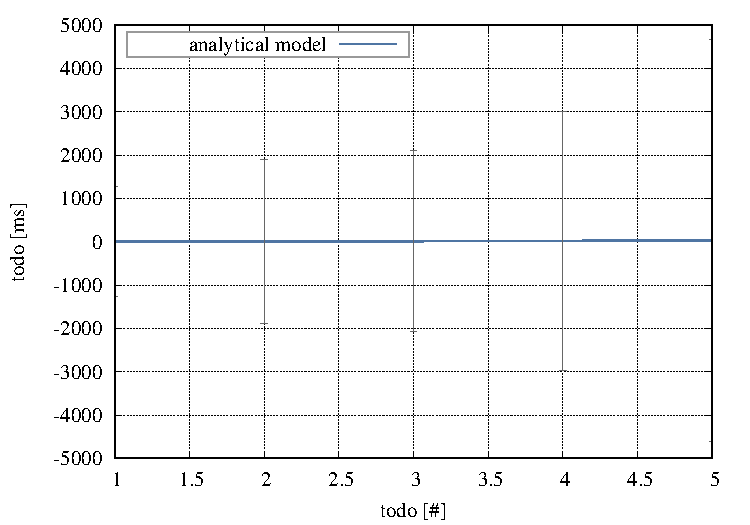
\includegraphics[width=.55\textwidth]{resources/images/example1}
    \caption{Example (based on~\cite{li2002design})}\label{fig:intro:a}
\end{figure}

\sidenote{Application Area: Foo Fooli}\index{Foo!Fooli}
\todomid{write about the application area~\cite{Heflin2004}}

\begin{figure}[H]
      \centering
      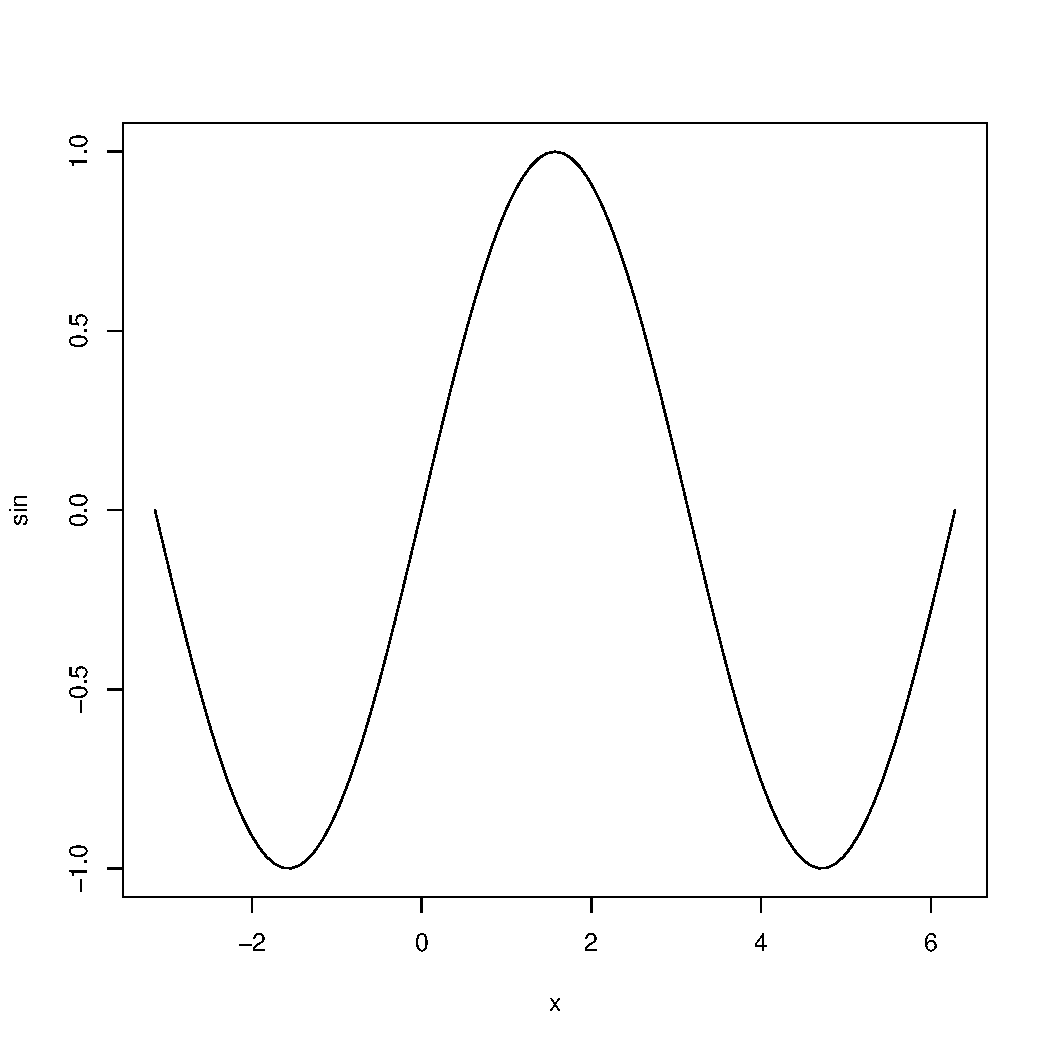
\includegraphics[width=.45\textwidth]{resources/images/example2}
      \caption{Another example~\cite{li2002design}}\label{fig:intro:b}
\end{figure}

\sidenote{Research Focus: Bar Barli}\index{Bar!Barli}
\todomid{write about the research focus and \Cref{fig:intro:b}}

\sidenote{Taxonomy}\index{Taxonomy}
\todomid{write about the taxonomy and \ac{ABAC}}

\begin{figure}[htbp]
      \centering
      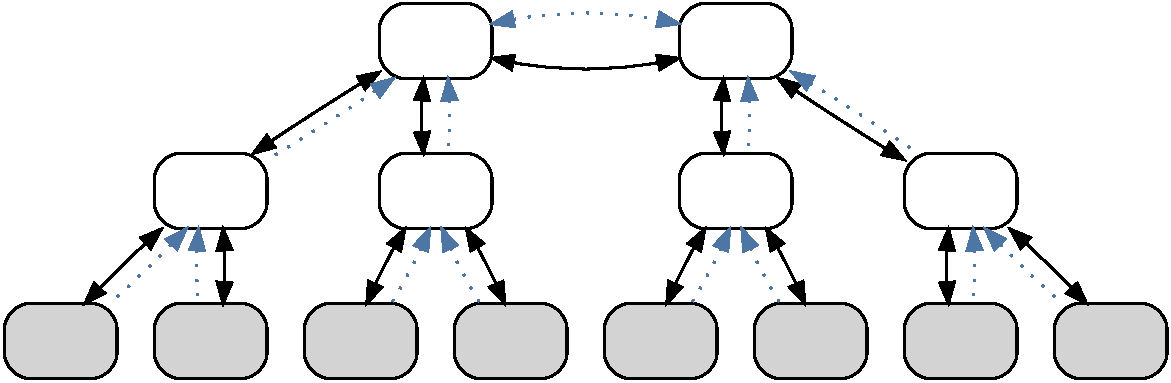
\includegraphics[width=.75\textwidth]{resources/images/example3}
      \caption{Taxonomy}
\end{figure}

\section{Problem Statement}\index{Requirements}

\sidenote{State of the Art}
\todomid{write about the State of the Art}

\sidenote{Issue:\\Example 1}
\todomid{write about the first issue}

\sidenote{Issue:\\Example 2}
\todomid{write about the second issue}

\sidenote{Synopsis}
\todomid{write about the synopsis of the issues and \Cref{fig:intro:c}}

\begin{figure}[htbp]
    \centering
    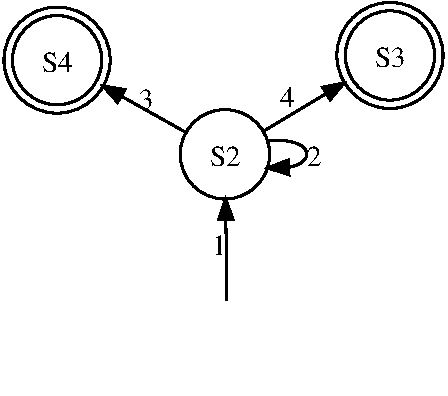
\includegraphics[width=.5\textwidth]{resources/images/job_lifecycle}
    \caption{Relationship between issues}\label{fig:intro:c}
\end{figure}

\section{Assumptions and Scope}

\sidenote{Research Assumptions}
\todomid{write about the research assumptions~\cite{li2002design}}

\sidenote{Research Scope}
\todomid{write about the research scope --- \Cref{fig:intro:a,fig:intro:b,fig:intro:c}}


\section{Objectives and Contributions}

\begin{figure}[htbp]
    \centering
    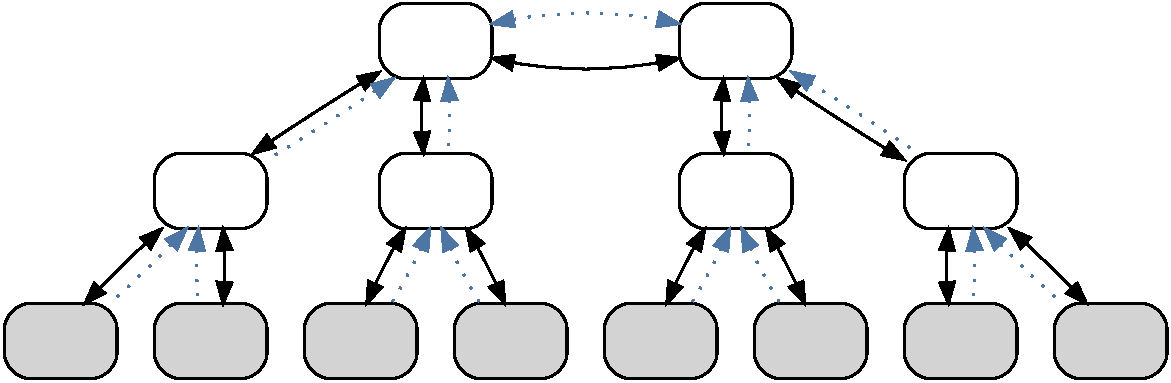
\includegraphics[width=.55\textwidth]{resources/images/example3}
    \caption{Structure of research}\label{fig:intro:struct}
\end{figure}

\sidenote{Research Objectives \& Contributions}
\todomid{write about the research objectives and \aclu{DBpedia} and \Cref{fig:intro:struct}}

\section{Methodology and Outline}

\todomid{write about the research outline and \Cref{fig:intro:methodology}. Summarize \Cref{sec:introduction,sec:sota,sec:reqs,sec:contrib1,sec:contrib2,sec:contrib3,sec:eval,sec:summary}.}

\begin{sidewaysfigure}
    \centering
    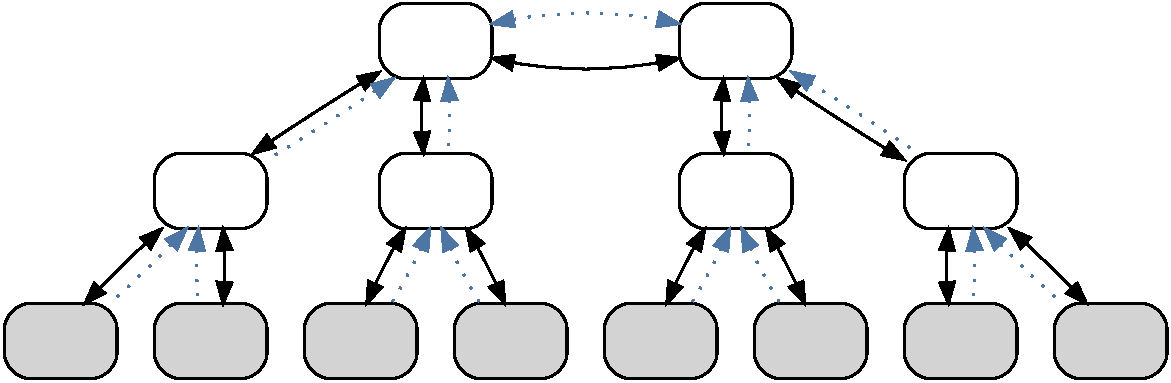
\includegraphics[width=.7\textwidth]{resources/images/example3}
    \caption{Workflow of the research and structure of the thesis}\label{fig:intro:methodology}
\end{sidewaysfigure}

    \cleardoublepage\chapter{State of the Art}\label{sec:sota}\minitoc\vspace{.5cm}\index{SotA}

\section{Introduction}

\begin{wrapfigure}{r}{0.2\textwidth}
    \centering
    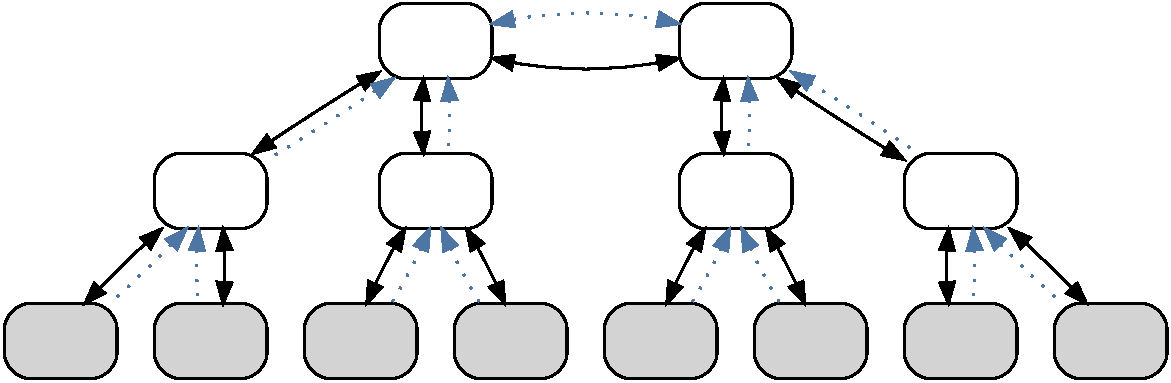
\includegraphics[width=0.2\textwidth]{resources/images/example3}
\end{wrapfigure}

\sidenote{Overview}
\todomid{write}

\section{Related Area 1}\index{Related Area}

\begin{figure}[H]
    \centering
    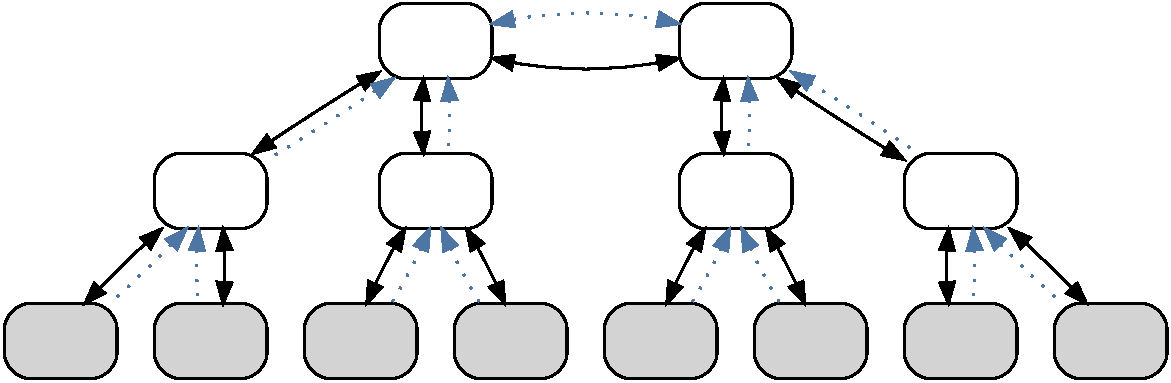
\includegraphics[width=.55\textwidth]{resources/images/example3}
    \caption{Related area 1 within the structure of research}\label{fig:hourglass:ra1}
\end{figure}

\sidenote{Overview}
\todomid{write about \Cref{fig:hourglass:ra1}}

\sidenote{Focus}
\todomid{write}

\subsection{Specific Example 1}

\sidenote{Definition}
\todomid{write}

\sidenote{Issues}
\todomid{write}

\subsection{Specific Example 2}

\sidenote{Definition}
\todomid{write}

\sidenote{Implementations}
\todomid{write}

\sidenote{Research}
\todomid{write}

\sidenote{Standards}
\todomid{write}

\sidenote{Adoption}
\todomid{write}

\subsection{Specific Example 3}\index{Example 3}

\sidenote{Transition}
\todomid{write about \Cref{fig:sota:trans}}

\begin{figure}
    \centering
    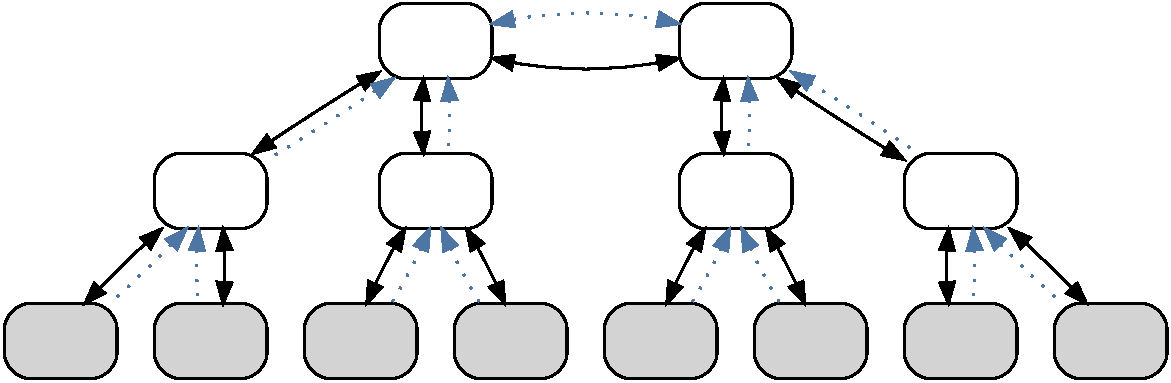
\includegraphics[width=.85\textwidth]{resources/images/example3}
    \caption{Comparison of Example 2 and Example 3 (based on~\cite{li2002design})}\label{fig:sota:trans}
\end{figure}

\sidenote{Standards}
\todomid{write}

\sidenote{Extension}
\todomid{write}

\sidenote{Other Standards}
\todomid{write}

\sidenote{Something}
\todomid{write}

\sidenote{Something}
\todomid{write}

\sidenote{Something}
\todomid{write}

\sidenote{Something}
\todomid{write}

\sidenote{Something}
\todomid{write}

\sidenote{Something}
\todomid{write}

\section{Related Area 2}\index{Related Area 2}

\sidenote{Overview}
\todomid{write}

\sidenote{Focus}
\todomid{write about \Cref{fig:sota:ra2}}

\begin{figure}[!hbtp]
    \centering
    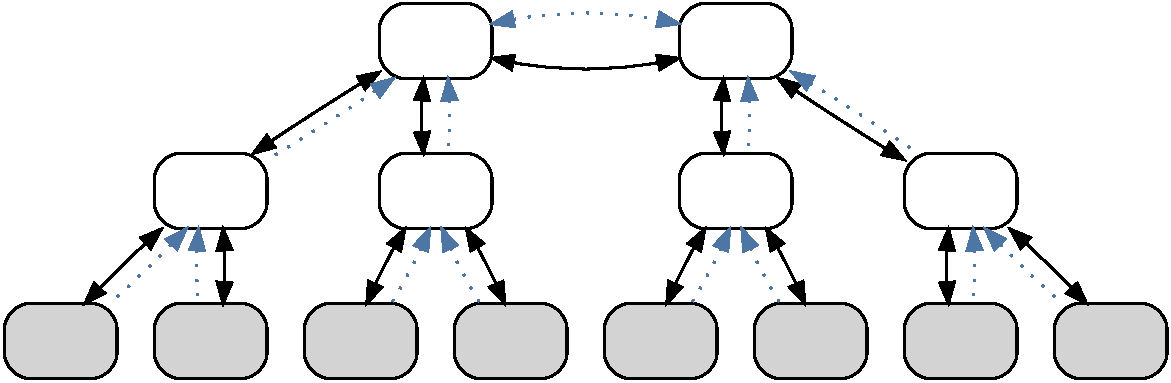
\includegraphics[width=1\textwidth]{resources/images/example3}
    \caption{Related Area 2}\label{fig:sota:ra2}
\end{figure}

\sidenote{Something}
\todomid{write}

\subsection{Specific Example 1}

\sidenote{Definition}
\todomid{write}

\sidenote{Issues}
\todomid{write}

\subsection{Specific Example 2}

\sidenote{Definition}
\todomid{write}

\sidenote{Implementations}
\todomid{write}

\sidenote{Research}
\todomid{write}

\sidenote{Standards}
\todomid{write}

\sidenote{Adoption}
\todomid{write}


\section{Related Area 3}\index{Related Area 3}

\sidenote{Overview}
\todomid{write}

\sidenote{Focus}
\todomid{write about \Cref{fig:sota:ra3}}

\begin{figure}[!hbtp]
    \centering
    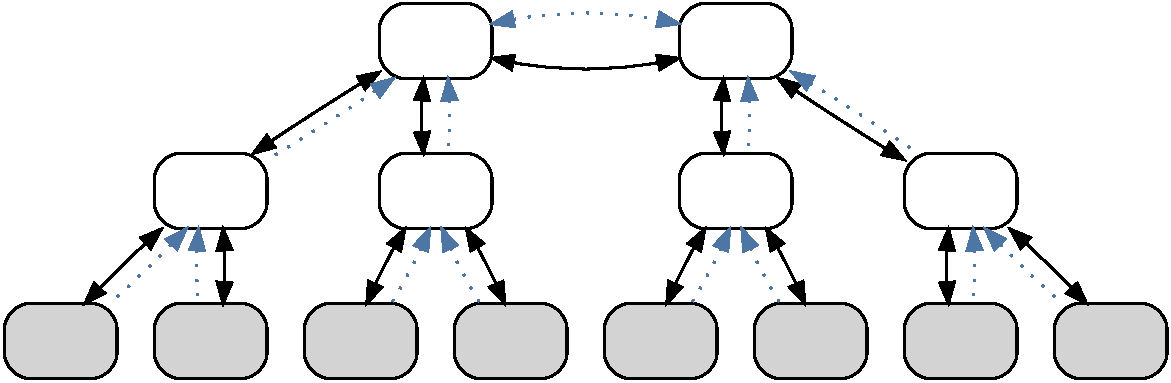
\includegraphics[width=1\textwidth]{resources/images/example3}
    \caption{Related Area 3}\label{fig:sota:ra3}
\end{figure}

\sidenote{Something}
\todomid{write}

\subsection{Specific Example 1}

\sidenote{Definition}
\todomid{write}

\sidenote{Issues}
\todomid{write}

\subsection{Specific Example 2}

\sidenote{Definition}
\todomid{write}

\sidenote{Implementations}
\todomid{write}

\sidenote{Research}
\todomid{write}

\sidenote{Standards}
\todomid{write}

\sidenote{Adoption}
\todomid{write}

\section{Conclusion}

\sidenote{Summary}
\todomid{write}

\sidenote{Takeaway 1}
\todomid{write}

\sidenote{Takeaway 2}
\todomid{write}

\sidenote{Takeaway 3}
\todomid{write}

\sidenote{Next chapter}
\todomid{write}

    \cleardoublepage
\chapter{Requirement Analysis}\label{sec:reqs}\minitoc\vspace{.5cm}
\index{Requirements}

\section{Introduction}

\begin{wrapfigure}{r}{0.2\textwidth}
    \centering
    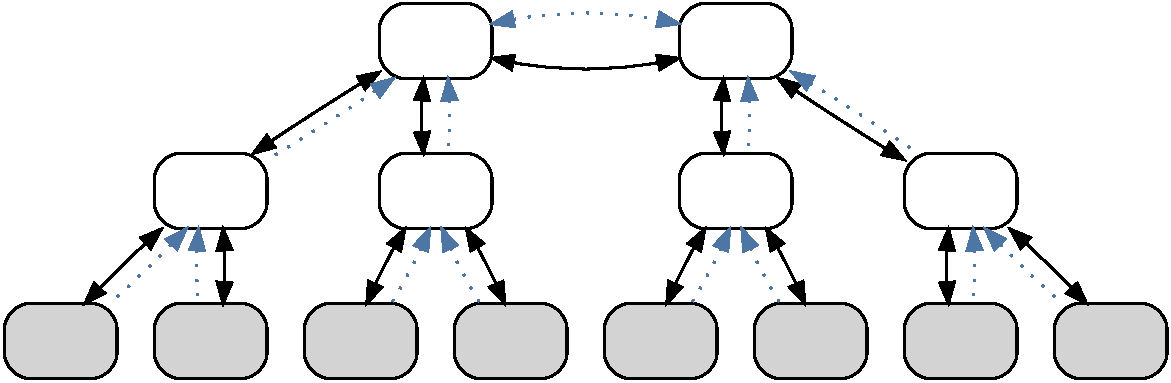
\includegraphics[width=0.2\textwidth]{resources/images/example3}
\end{wrapfigure}

\sidenote{Overview}
\todomid{write about \Cref{fig:req:details}}

\begin{figure}[H]
    \centering
    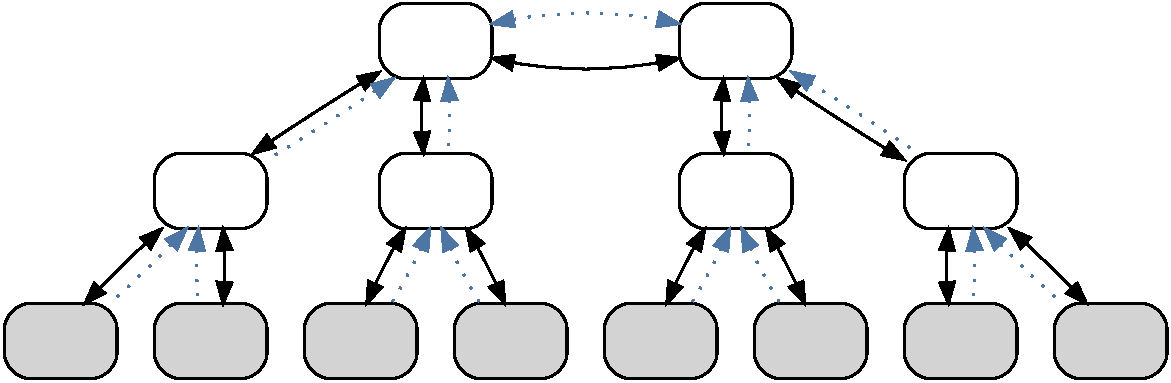
\includegraphics[width=.85\textwidth]{resources/images/example3}
    \caption{More detailed overview of the requirements}\label{fig:req:details}
\end{figure}

\sidenote{Structure of Research}
\todomid{write about \Cref{fig:hourglass:reqs}}

\begin{figure}[H]
    \centering
    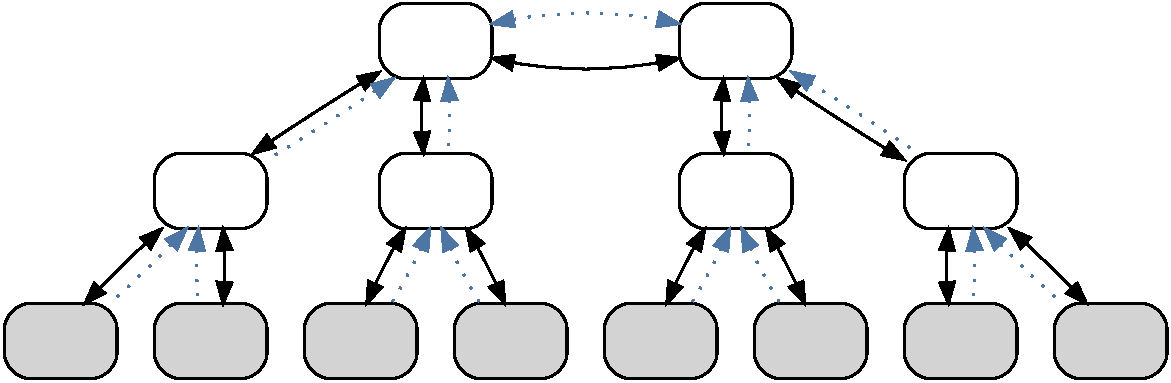
\includegraphics[width=.55\textwidth]{resources/images/example3}
    \caption{Placement of the requirement section in the structure of research}\label{fig:hourglass:reqs}
\end{figure}

\section{Stakeholder 1}

\sidenote{\Cref{tbl:reqs:stakeholder1}}
\todomid{write about \Cref{tbl:reqs:stakeholder1}}

\begin{tabularx}{\textwidth}{lX}
    \caption{Requirements from stakeholder 1 perspective}\label{tbl:reqs:stakeholder1}\\
    \toprule
    \textbf{\#}& \textbf{Description}  \\\midrule
    \endfirsthead%
    \toprule
    \textbf{\#}& \textbf{Description}  \\\midrule
    \endhead%
    \requirement{U}{req:stakeholder1:foo}{Foo}
       & \todomid{write}
    \\\midrule
    \requirement{U}{req:stakeholder1:bar}{Bar}
       & \todomid{write}
    \\\bottomrule
\end{tabularx}

\section{Stakeholder 2}

\sidenote{\Cref{tbl:reqs:stakeholder2}}
\todomid{write about \Cref{tbl:reqs:stakeholder2}}

\begin{tabularx}{\textwidth}{lX}
    \caption{Requirements from stakeholder 2 perspective}\label{tbl:reqs:stakeholder2}\\
    \toprule
    \textbf{\#}& \textbf{Description}  \\\midrule
    \endfirsthead%
    \toprule
    \textbf{\#}& \textbf{Description}  \\\midrule
    \endhead%
    \requirement{S}{req:stakeholder2:foo}{Foo}
       & \todomid{write}
    \\\midrule
    \requirement{S}{req:stakeholder2:bar}{Bar}
       & \todomid{write}
    \\\bottomrule
\end{tabularx}

\section{Stakeholder 3}

\sidenote{\Cref{tbl:reqs:stakeholder3}}
\todomid{write about \Cref{tbl:reqs:stakeholder3}}

\begin{tabularx}{\textwidth}{lX}
    \caption{Requirements from stakeholder 3 perspective}\label{tbl:reqs:stakeholder3}\\
    \toprule
    \textbf{\#}& \textbf{Description}  \\\midrule
    \endfirsthead%
    \toprule
    \textbf{\#}& \textbf{Description}  \\\midrule
    \endhead%
    \requirement{T}{req:stakeholder3:foo}{Foo}
       & \todomid{write}
    \\\midrule
    \requirement{T}{req:stakeholder3:bar}{Bar}
       & \todomid{write}
    \\\bottomrule
\end{tabularx}

\section{Conclusion}

\sidenote{Summary}
\todomid{write}

\sidenote{Takeaway 1}
\todomid{write}

\sidenote{Takeaway 2}
\todomid{write}

\sidenote{Takeaway 3}
\todomid{write}

\sidenote{Next chapter}
\todomid{write}

    \cleardoublepage
\chapter{Contribution 1}\label{sec:contrib1}\minitoc\vspace{.5cm}
\index{Contribution 1}

\section{Introduction}

\begin{wrapfigure}{r}{0.2\textwidth}
    \centering
    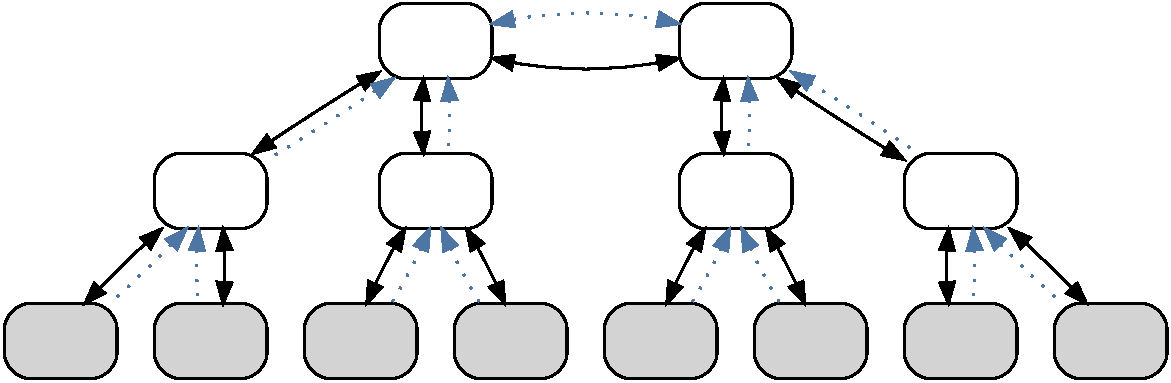
\includegraphics[width=0.2\textwidth]{resources/images/example3}
\end{wrapfigure}

\sidenote{Overview}
\todomid{write}

\sidenote{Structure of Research}
\todomid{write about \Cref{fig:hourglass:contrib1}}

\begin{figure}[H]
    \centering
    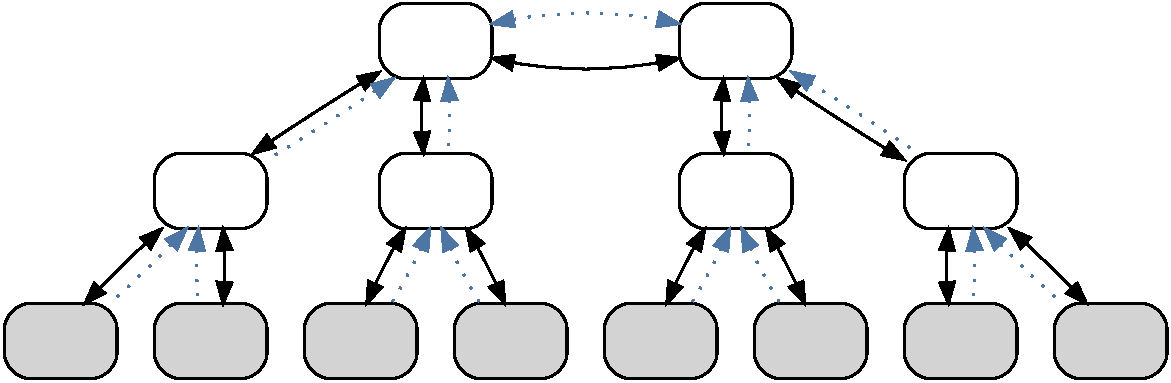
\includegraphics[width=.55\textwidth]{resources/images/example3}
    \caption{Placement of contribution 1 in the structure of research}\label{fig:hourglass:contrib1}
\end{figure}

\section{State of the Art}

\sidenote{Overview}
\todomid{write about \Cref{fig:contrib1:related}}

\begin{figure}[htbp]
    \centering
    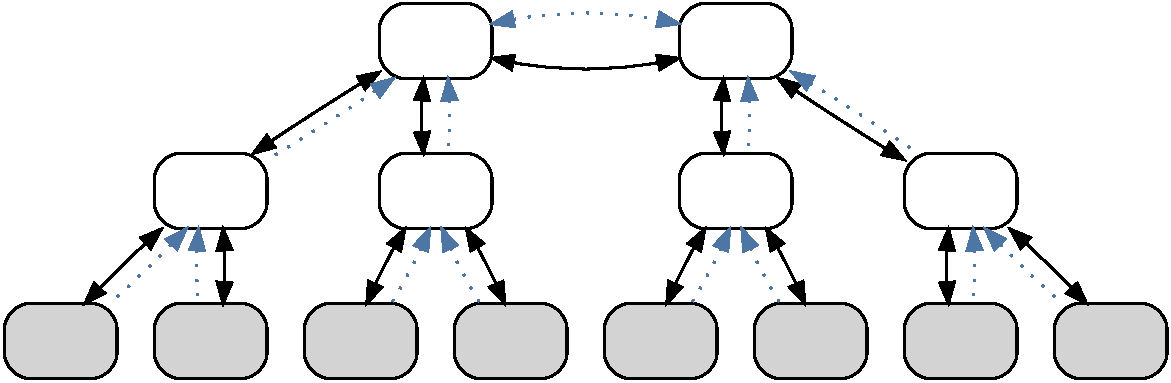
\includegraphics[width=.6\textwidth]{resources/images/example3}
    \caption{Relationship of contribution 1 to related work}\label{fig:contrib1:related}
\end{figure}

\subsection{Related Work 1}

\sidenote{Overview}
\todomid{write}

\sidenote{Some Aspects}
\todomid{write}

\sidenote{Issues}
\todomid{write about \Cref{lst:contrib1:rw1}}

\lstset{caption=Listing related to related work 1 for contribution 1, label=lst:contrib1:rw1,
language=xml, breaklines=true, numbers=left, basicstyle=\small\ttfamily,
stepnumber=1, frame=single, inputencoding=utf8/latin1}~\lstinputlisting{resources/code/example.java}

\subsection{Related Work 2}

\sidenote{Overview}
\todomid{write}

\sidenote{Some Aspects}
\todomid{write}

\sidenote{Issues}
\todomid{write about \Cref{lst:contrib1:rw2}}

\lstset{caption=Listing related to related work 2 for contribution 1, label=lst:contrib1:rw2,
language=xml, breaklines=true, numbers=left, basicstyle=\small\ttfamily,
stepnumber=1, frame=single, inputencoding=utf8/latin1}~\lstinputlisting{resources/code/example.java}

\subsection{Related Work 3}

\sidenote{Overview}
\todomid{write}

\sidenote{Some Aspects}
\todomid{write}

\sidenote{Issues}
\todomid{write about \Cref{lst:contrib1:rw3}}

\lstset{caption=Listing related to related work 3 for contribution 1, label=lst:contrib1:rw3,
language=xml, breaklines=true, numbers=left, basicstyle=\small\ttfamily,
stepnumber=1, frame=single, inputencoding=utf8/latin1}~\lstinputlisting{resources/code/example.java}


\section{Own Approach}

\subsection{Overview}

\sidenote{Intro}
\todomid{write}

\sidenote{Goal}
\todomid{write about \Cref{fig:contrib1:goal}}

\begin{figure}[htbp]
    \centering
    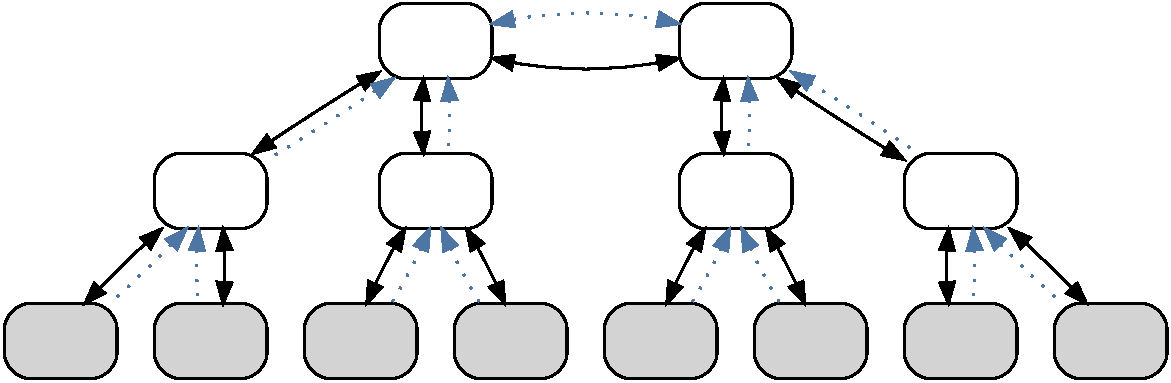
\includegraphics[width=.95\textwidth]{resources/images/example3}
    \caption{Contribution 1 goal}\label{fig:contrib1:goal}
\end{figure}

\sidenote{Approach}
\todomid{write}

\subsection{First Part}

\sidenote{Overview}
\todomid{write}

\sidenote{Approach}
\todomid{write}

\sidenote{Integration}
\todomid{write}

\subsection{Second Part}

\sidenote{Overview}
\todomid{write}

\sidenote{Approach}
\todomid{write}

\sidenote{Integration}
\todomid{write}

\subsection{Third Part}

\sidenote{Overview}
\todomid{write}

\sidenote{Approach}
\todomid{write}

\sidenote{Integration}
\todomid{write}

\section{Conclusion}

\sidenote{Summary}
\todomid{write}

\sidenote{Takeaway 1}
\todomid{write}

\sidenote{Takeaway 2}
\todomid{write}

\sidenote{Takeaway 3}
\todomid{write}

\sidenote{Next chapter}
\todomid{write}

    \cleardoublepage
\chapter{Contribution 2}\label{sec:contrib2}\minitoc\vspace{.5cm}
\index{Contribution 2}

\section{Introduction}

\begin{wrapfigure}{r}{0.2\textwidth}
    \centering
    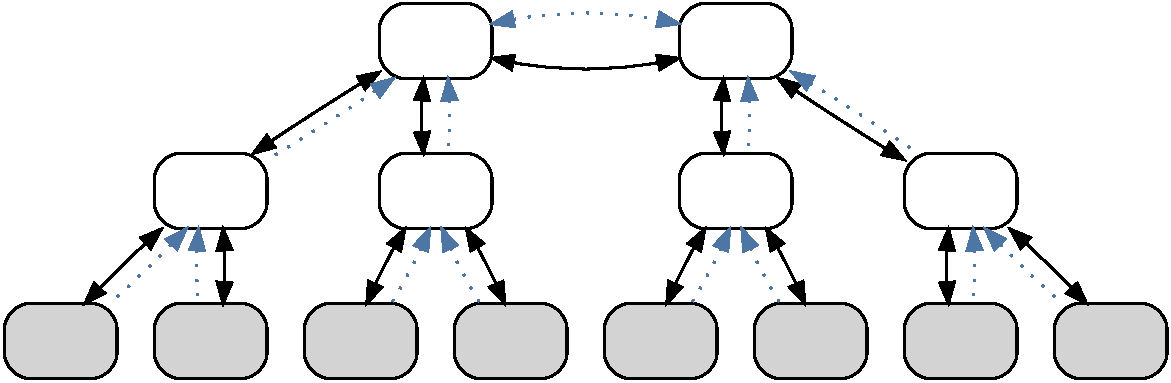
\includegraphics[width=0.2\textwidth]{resources/images/example3}
\end{wrapfigure}

\sidenote{Overview}
\todomid{write}

\sidenote{Structure of Research}
\todomid{write about \Cref{fig:hourglass:contrib2}}

\begin{figure}[H]
    \centering
    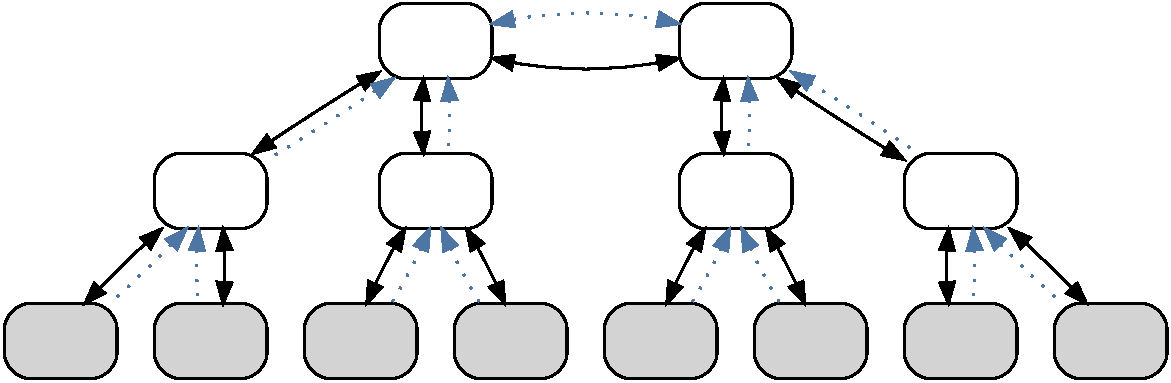
\includegraphics[width=.55\textwidth]{resources/images/example3}
    \caption{Placement of Contribution 2 in the structure of research}\label{fig:hourglass:contrib2}
\end{figure}

\section{State of the Art}

\sidenote{Overview}
\todomid{write about \Cref{fig:contrib2:related}}

\begin{figure}[htbp]
    \centering
    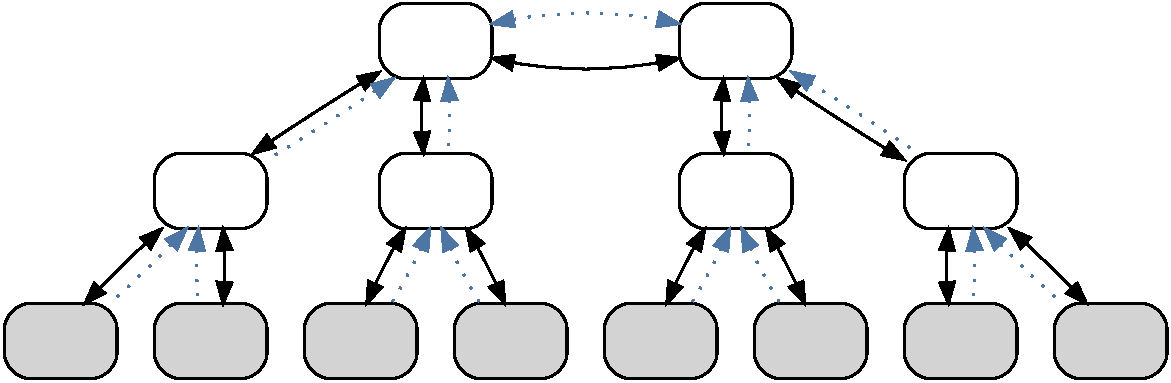
\includegraphics[width=.6\textwidth]{resources/images/example3}
    \caption{Relationship of Contribution 2 to related work}\label{fig:contrib2:related}
\end{figure}

\subsection{Related Work 1}

\sidenote{Overview}
\todomid{write}

\sidenote{Some Aspects}
\todomid{write}

\sidenote{Issues}
\todomid{write about \Cref{lst:contrib2:rw1}}

\lstset{caption=Listing related to related work 1 for Contribution 2, label=lst:contrib2:rw1,
language=xml, breaklines=true, numbers=left, basicstyle=\small\ttfamily,
stepnumber=1, frame=single, inputencoding=utf8/latin1}~\lstinputlisting{resources/code/example.java}

\subsection{Related Work 2}

\sidenote{Overview}
\todomid{write}

\sidenote{Some Aspects}
\todomid{write}

\sidenote{Issues}
\todomid{write about \Cref{lst:contrib2:rw2}}

\lstset{caption=Listing related to related work 2 for Contribution 2, label=lst:contrib2:rw2,
language=xml, breaklines=true, numbers=left, basicstyle=\small\ttfamily,
stepnumber=1, frame=single, inputencoding=utf8/latin1}~\lstinputlisting{resources/code/example.java}

\subsection{Related Work 3}

\sidenote{Overview}
\todomid{write}

\sidenote{Some Aspects}
\todomid{write}

\sidenote{Issues}
\todomid{write about \Cref{lst:contrib2:rw3}}

\lstset{caption=Listing related to related work 3 for Contribution 2, label=lst:contrib2:rw3,
language=xml, breaklines=true, numbers=left, basicstyle=\small\ttfamily,
stepnumber=1, frame=single, inputencoding=utf8/latin1}~\lstinputlisting{resources/code/example.java}


\section{Own Approach}

\subsection{Overview}

\sidenote{Intro}
\todomid{write}

\sidenote{Goal}
\todomid{write about \Cref{fig:contrib2:goal}}

\begin{figure}[htbp]
    \centering
    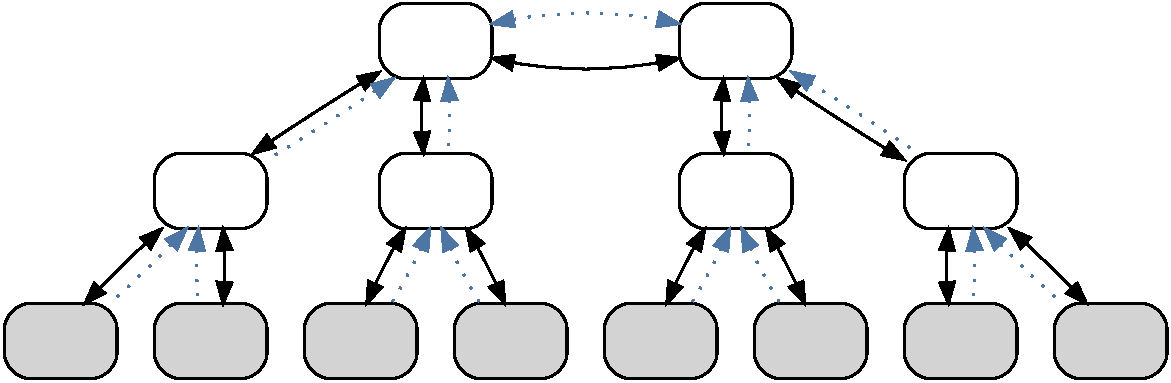
\includegraphics[width=.95\textwidth]{resources/images/example3}
    \caption{Contribution 2 goal}\label{fig:contrib2:goal}
\end{figure}

\sidenote{Approach}
\todomid{write}

\subsection{First Part}

\sidenote{Overview}
\todomid{write}

\sidenote{Approach}
\todomid{write}

\sidenote{Integration}
\todomid{write}

\subsection{Second Part}

\sidenote{Overview}
\todomid{write}

\sidenote{Approach}
\todomid{write}

\sidenote{Integration}
\todomid{write}

\subsection{Third Part}

\sidenote{Overview}
\todomid{write}

\sidenote{Approach}
\todomid{write}

\sidenote{Integration}
\todomid{write}

\section{Conclusion}

\sidenote{Summary}
\todomid{write}

\sidenote{Takeaway 1}
\todomid{write}

\sidenote{Takeaway 2}
\todomid{write}

\sidenote{Takeaway 3}
\todomid{write}

\sidenote{Next chapter}
\todomid{write}

    \cleardoublepage
\chapter{Contribution 3}\label{sec:contrib3}\minitoc\vspace{.5cm}
\index{Contribution 3}

\section{Introduction}

\begin{wrapfigure}{r}{0.2\textwidth}
    \centering
    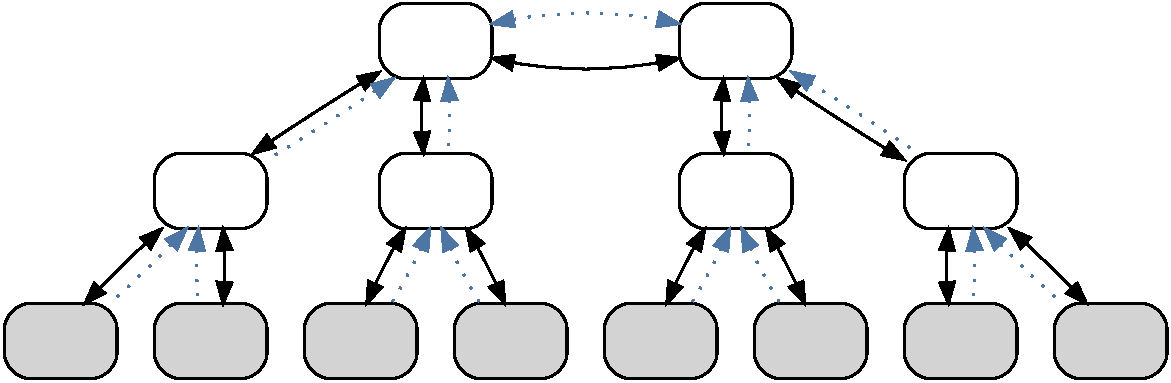
\includegraphics[width=0.2\textwidth]{resources/images/example3}
\end{wrapfigure}

\sidenote{Overview}
\todomid{write}

\sidenote{Structure of Research}
\todomid{write about \Cref{fig:hourglass:contrib3}}

\begin{figure}[H]
    \centering
    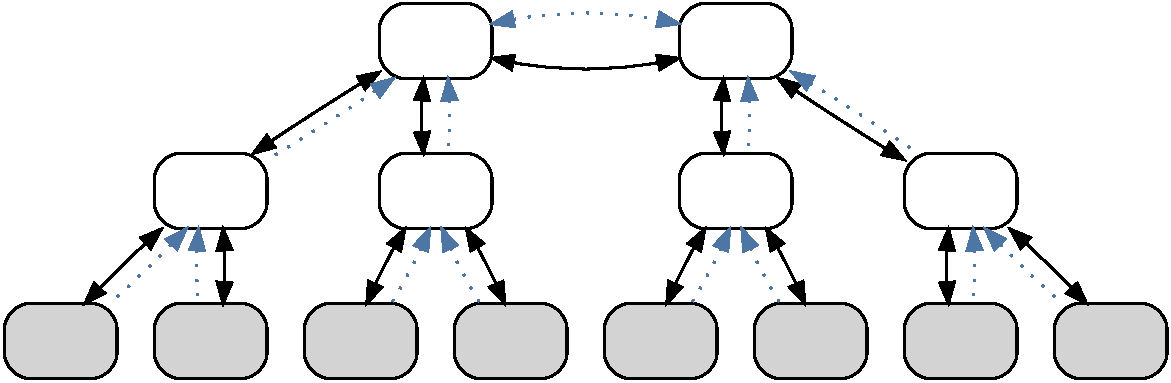
\includegraphics[width=.55\textwidth]{resources/images/example3}
    \caption{Placement of Contribution 3 in the structure of research}\label{fig:hourglass:contrib3}
\end{figure}

\section{State of the Art}

\sidenote{Overview}
\todomid{write about \Cref{fig:contrib3:related}}

\begin{figure}[htbp]
    \centering
    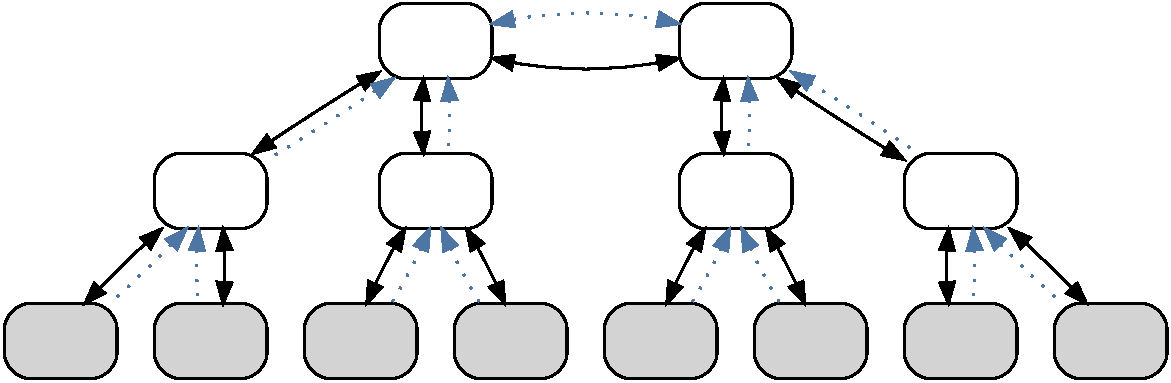
\includegraphics[width=.6\textwidth]{resources/images/example3}
    \caption{Relationship of Contribution 3 to related work}\label{fig:contrib3:related}
\end{figure}

\subsection{Related Work 1}

\sidenote{Overview}
\todomid{write}

\sidenote{Some Aspects}
\todomid{write}

\sidenote{Issues}
\todomid{write about \Cref{lst:contrib3:rw1}}

\lstset{caption=Listing related to related work 1 for Contribution 3, label=lst:contrib3:rw1,
language=xml, breaklines=true, numbers=left, basicstyle=\small\ttfamily,
stepnumber=1, frame=single, inputencoding=utf8/latin1}~\lstinputlisting{resources/code/example.java}

\subsection{Related Work 2}

\sidenote{Overview}
\todomid{write}

\sidenote{Some Aspects}
\todomid{write}

\sidenote{Issues}
\todomid{write about \Cref{lst:contrib3:rw2}}

\lstset{caption=Listing related to related work 2 for Contribution 3, label=lst:contrib3:rw2,
language=xml, breaklines=true, numbers=left, basicstyle=\small\ttfamily,
stepnumber=1, frame=single, inputencoding=utf8/latin1}~\lstinputlisting{resources/code/example.java}

\subsection{Related Work 3}

\sidenote{Overview}
\todomid{write}

\sidenote{Some Aspects}
\todomid{write}

\sidenote{Issues}
\todomid{write about \Cref{lst:contrib3:rw3}}

\lstset{caption=Listing related to related work 3 for Contribution 3, label=lst:contrib3:rw3,
language=xml, breaklines=true, numbers=left, basicstyle=\small\ttfamily,
stepnumber=1, frame=single, inputencoding=utf8/latin1}~\lstinputlisting{resources/code/example.java}


\section{Own Approach}

\subsection{Overview}

\sidenote{Intro}
\todomid{write}

\sidenote{Goal}
\todomid{write about \Cref{fig:contrib3:goal}}

\begin{figure}[htbp]
    \centering
    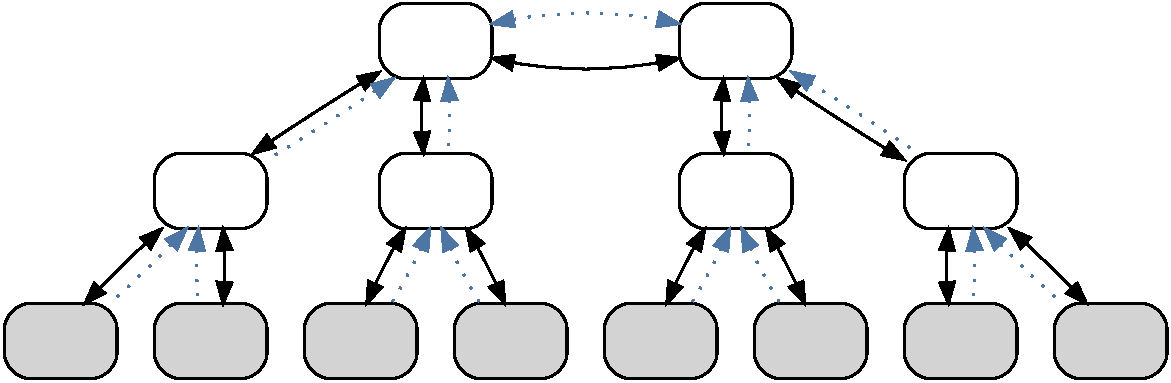
\includegraphics[width=.95\textwidth]{resources/images/example3}
    \caption{Contribution 3 goal}\label{fig:contrib3:goal}
\end{figure}

\sidenote{Approach}
\todomid{write}

\subsection{First Part}

\sidenote{Overview}
\todomid{write}

\sidenote{Approach}
\todomid{write}

\sidenote{Integration}
\todomid{write}

\subsection{Second Part}

\sidenote{Overview}
\todomid{write}

\sidenote{Approach}
\todomid{write}

\sidenote{Integration}
\todomid{write}

\subsection{Third Part}

\sidenote{Overview}
\todomid{write}

\sidenote{Approach}
\todomid{write}

\sidenote{Integration}
\todomid{write}

\section{Conclusion}

\sidenote{Summary}
\todomid{write}

\sidenote{Takeaway 1}
\todomid{write}

\sidenote{Takeaway 2}
\todomid{write}

\sidenote{Takeaway 3}
\todomid{write}

\sidenote{Next chapter}
\todomid{write}

    \cleardoublepage
\chapter{Evaluation}\label{sec:eval}\minitoc\vspace{.5cm}
\index{Evaluation}\index{Validation}\index{Verification}

\section{Introduction}

\begin{wrapfigure}{r}{0.2\textwidth}
    \centering
    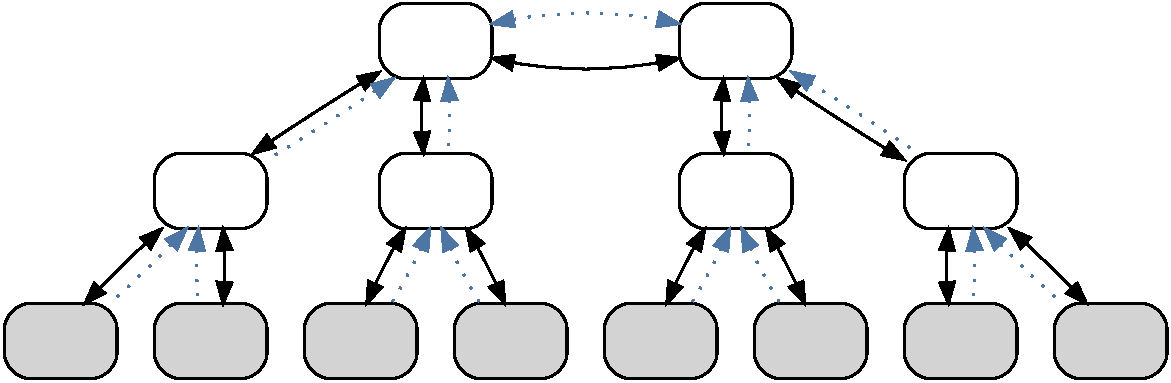
\includegraphics[width=0.2\textwidth]{resources/images/example3}
\end{wrapfigure}

\sidenote{Overview}
\todomid{write about \Cref{sec:eval:tec}}

\begin{figure}[htbp]
    \centering
    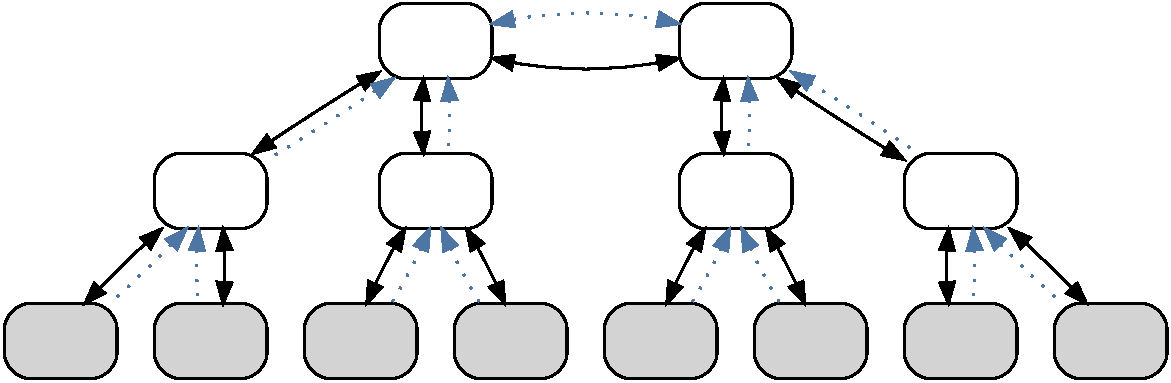
\includegraphics[width=.8\textwidth]{resources/images/example3}
    \caption{Choice of verification and validation techniques~\cite{li2002design}}\label{sec:eval:tec}
\end{figure}

\sidenote{Approaches}
\todomid{write}

\sidenote{Structure of Research}
\todomid{write about \Cref{fig:hourglass:evaluation}}

\begin{figure}[htpb]
    \centering
    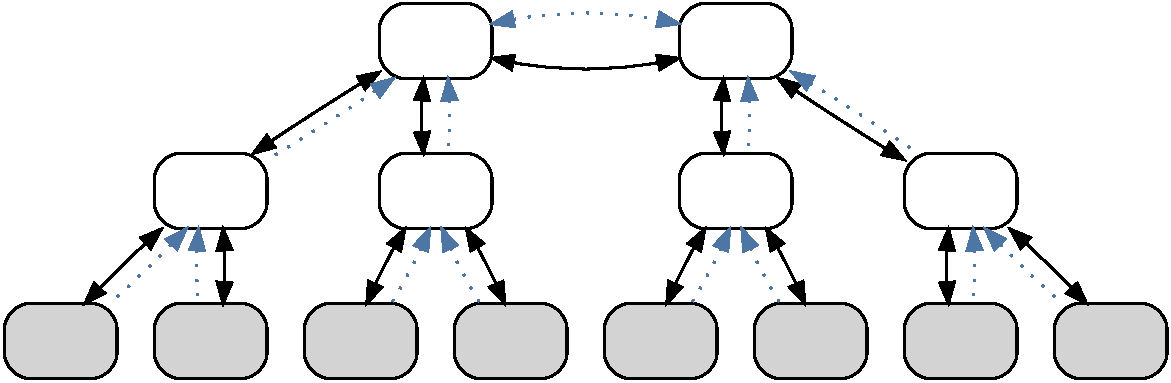
\includegraphics[width=.55\textwidth]{resources/images/example3}
    \caption{Placement of the evaluation in the structure of research}\label{fig:hourglass:evaluation}
\end{figure}

\section{Experimental Validation}

\sidenote{Overview}
\todomid{write about \Cref{tbl:eval:experiments}}

\begin{sidewaystable}
      \centering
      \captionsetup{type=table}
      \caption{Sideways table}
      \begin{tabular}{lllllll}\toprule
  \textbf{Experiment 1}   & \textbf{Experiment 2}  & \textbf{Experiment 3} & \textbf{Experiment 4} & \textbf{Experiment 5} & \textbf{Experiment 6} & \textbf{Experiment 7}  \\ \midrule
  CATCH & ME & IF & YOU & CAN & \emph{NOW} & OR NEVER \\
  CATCH & ME & IF & YOU & CAN & \emph{NOW} & OR NEVER \\
  CATCH & ME & IF & YOU & CAN & \emph{NOW} & OR NEVER \\
  CATCH & ME & IF & YOU & CAN & \emph{NOW} & OR NEVER \\
  CATCH & ME & IF & YOU & CAN & \emph{NOW} & OR NEVER \\
  CATCH & ME & IF & YOU & CAN & \emph{NOW} & OR NEVER \\
  CATCH & ME & IF & YOU & CAN & \emph{NOW} & OR NEVER \\
  CATCH & ME & IF & YOU & CAN & \emph{NOW} & OR NEVER \\
  CATCH & ME & IF & YOU & CAN & \emph{NOW} & OR NEVER \\
  CATCH & ME & IF & YOU & CAN & \emph{NOW} & OR NEVER \\
  CATCH & ME & IF & YOU & CAN & \emph{NOW} & OR NEVER \\
  \bottomrule
      \end{tabular}\label{tbl:eval:experiments}
\end{sidewaystable}


\subsection{Setup 1}

\sidenote{Overview}
\todomid{write}

\sidenote{Integration}
\todomid{write about \Cref{eq:var_idb}}

\small
\begin{equation}
  \begin{array}{l}
    \displaystyle t^{p_d}_{fw}(d) = \max_{d}(t_{child_{i}}) \\
    \displaystyle t^{p_d}_{db}(d) = \sum_{i=1}^{d} t_{db_{i}} \\
    \displaystyle t^{p_d}_{pc}(n,d) =
    	\begin{cases}
        	t_{pc}(d) + c(n) & \text{if $d = 1$,}\\
        	t_{pc}(d) + c(n) + \max(t_{avail}(d)) & \text{if $d>1$.}\\
        \end{cases}
  \end{array}\label{eq:var_idb}
\end{equation}
\normalsize

\sidenote{Example}
\todomid{write about \Cref{lst:eval:exp1}}

\needspace{5\baselineskip}\lstset{caption=Experiment 1, label=lst:eval:exp1,
language=ttl, breaklines=true, numbers=left,
stepnumber=1, frame=single, inputencoding=utf8/latin1}~\lstinputlisting{resources/code/example.java}

\subsection{Setup 2}

\sidenote{Overview}
\todomid{write}

\sidenote{Integration}
\todomid{write}

\sidenote{Example}
\todomid{write about \Cref{fig:eval:sub1,fig:eval:sub2,fig:eval:sub}}

\begin{figure}
    \begin{subfigure}[b]{.455\textwidth}
      \centering
      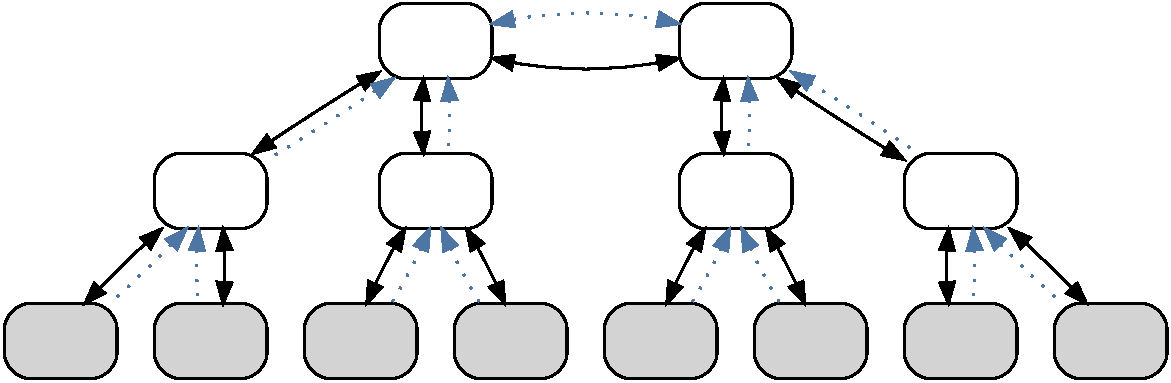
\includegraphics[width=.9\textwidth,frame]{resources/images/example3}
      \caption{Subfig 1}\label{fig:eval:sub1}
    \end{subfigure}~\begin{subfigure}[b]{.545\textwidth}
      \centering
      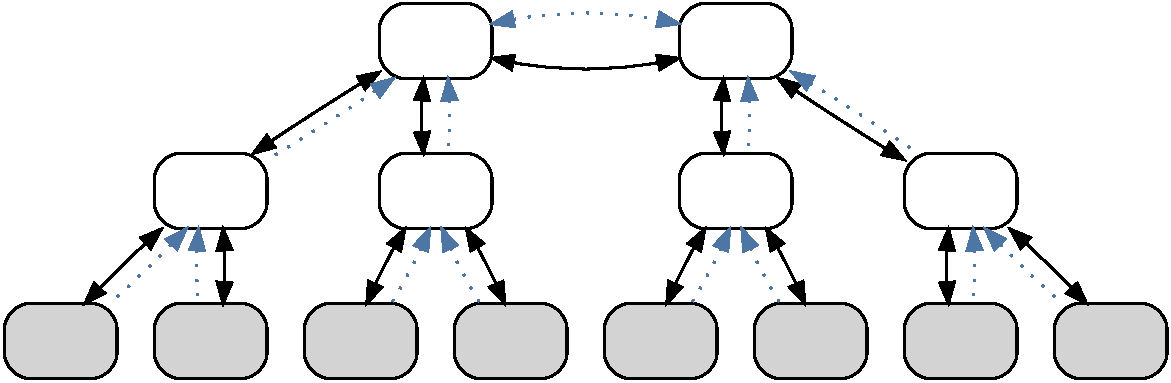
\includegraphics[width=1\textwidth,frame]{resources/images/example3}
      \caption{Subfig 2}\label{fig:eval:sub2}
    \end{subfigure}
    \caption{Sub Figures}\label{fig:eval:sub}
\end{figure}


\section{Performance Evaluation}

\sidenote{Overview}
\todomid{write}

\subsection{Evaluation 1}

\sidenote{Setup}
\todomid{write}

\sidenote{Cost Metrics}
\todomid{write}

\sidenote{Optimizing}
\todomid{write}

\sidenote{Performance Comparison}
\todomid{write}

\subsection{Evaluation 2}

\sidenote{Setup}
\todomid{write}

\sidenote{Response Times}
\todomid{write}
\begin{itemize}[noitemsep]
  \item \emph{In}: 159 ms $\pm$ 21 ms (95\% CI)
  \item \emph{Out}: 33 ms $\pm$ 5 ms (95\% CI)
  \item \emph{Between}: 238 ms $\pm$ 9 ms (95\% CI)
  \item \emph{After}: 45 ms $\pm$ 1 ms (95\% CI)
  \item \emph{Under}: 215 ms $\pm$ 2 ms (95\% CI)
  \item \emph{Over}: 148 ms $\pm$ 3 ms (95\% CI)
\end{itemize}

\sidenote{Scalability}
\todomid{write}

\section{Observational Validation}

\sidenote{Overview}
\todomid{write}

\subsection{Project 1}

\sidenote{Overview}
\todomid{write}

\sidenote{System Specification}
\todomid{write}

\sidenote{Extraction}
\todomid{write}

\sidenote{Example}
\todomid{write}

\subsection{Project 2}

\sidenote{Overview}
\todomid{write}

\sidenote{System Specification}
\todomid{write about \Cref{fig:eval:side}}

\begin{figure}[htbp]
    \centering
    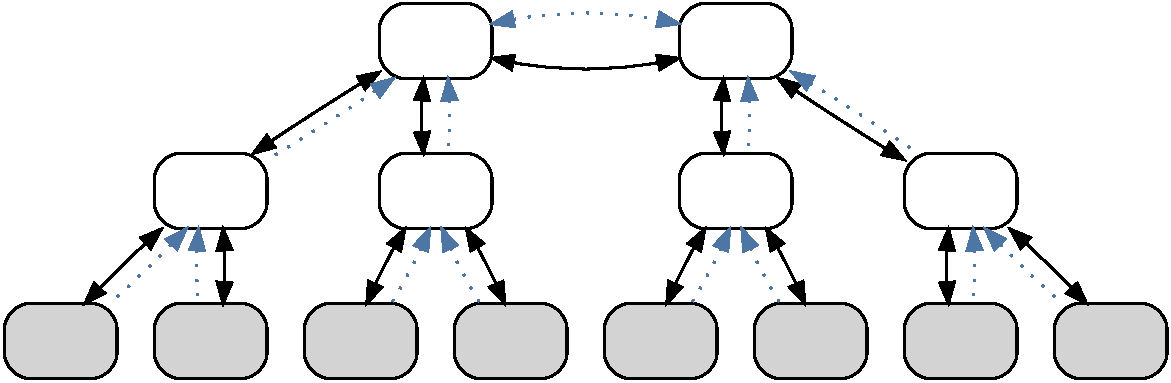
\includegraphics[height=.5\textwidth,angle=270]{resources/images/example3}
    \caption{Sideways figure}\label{fig:eval:side}
\end{figure}

\sidenote{Extraction}
\todomid{write}

\sidenote{Example}
\todomid{write}

\section{Deployments}

\sidenote{Overview}
\todomid{write}

\subsection{Installation 1}

\sidenote{Overview}
\todomid{write}

\sidenote{Integration}
\todomid{write}


\subsection{Installation 2}

\sidenote{Overview}
\todomid{write}

\sidenote{Integration}
\todomid{write}

\section{Code Verification}

\sidenote{Overview}
\todomid{write}

\sidenote{Static Tests}
\todomid{write}

\sidenote{Continuous Integration}
\todomid{write}

\sidenote{Test Coverage}
\todomid{write}

\section{Comparative Analysis}

\sidenote{Overview}
\todomid{write}

\subsection{Requirement Evaluation}

\sidenote{\Cref{tbl:reqs:compare}}
\todomid{write}

\begin{tabularx}{\textwidth}{p{2cm}X}
    \caption{Mapping requirements against own approach}\label{tbl:reqs:compare}\\
    \toprule
    \textbf{Requirements}& \textbf{Approach}  \\\midrule
    \endfirsthead%
    \toprule
    \textbf{Requirements}& \textbf{Approach}  \\\midrule
    \endhead%
\ref{req:stakeholder1:foo}\newline(Foo) &
\todomid{write}
\\\midrule

\ref{req:stakeholder1:bar}\newline(Bar) &
\todomid{write}
\\\midrule

\ref{req:stakeholder2:foo}\newline(Foo) &
\todomid{write}
\\\midrule

\ref{req:stakeholder2:bar}\newline(Bar) &
\todomid{write}
\\\midrule

\ref{req:stakeholder3:foo}\newline(Foo) &
\todomid{write}
\\\midrule

\ref{req:stakeholder3:bar}\newline(Bar) &
\todomid{write}

\\\bottomrule
\end{tabularx}

\subsection{Comparison with Other Approaches}

\sidenote{Overview}
\todomid{write}

\sidenote{\Cref{tbl:approaches:compare}}
\todomid{write about \Cref{tbl:approaches:compare}}

\begin{tabularx}{\textwidth}{p{2cm}LLLLLL}
    \caption{Comparison of related work with own approach}\label{tbl:approaches:compare}\\
    \toprule
    \textbf{Requirements} & \textbf{Related 1} & \textbf{Related 2} & \textbf{Related 3} & \textbf{Related 4} & \textbf{Related 5} & \textbf{Own Approach} \\\midrule
    \endfirsthead%
    \toprule
    \textbf{Requirements} & \textbf{Related 1} & \textbf{Related 2} & \textbf{Related 3} & \textbf{Related 4} & \textbf{Related 5} & \textbf{Own Approach} \\\midrule
    \endhead%

\ref{req:stakeholder1:foo}~\ref{req:stakeholder1:bar} & \textbf{(+)} & \textbf{(++)} & \textbf{(o)} & \textbf{(-)} & \textbf{(o)} & \textbf{(+++)} \\
(\ac{ABAC}) & \ac{ABAC} \ac{ABAC} v3, \ac{ABAC} \ac{ABAC} & \ac{ABAC} \ac{ABAC} v2, \ac{ABAC}, native \ac{ABAC} & \ac{ABAC} & native \ac{ABAC} & \ac{ABAC} \ac{ABAC} v2 & \ac{ABAC} \ac{ABAC} v3, \ac{ABAC} \ac{ABAC}, \ac{ABAC}, native \ac{ABAC}, native \\\midrule

\ref{req:stakeholder3:foo} & \textbf{(o)} & \textbf{(++)} &  & & \textbf{(++)} & \textbf{(+)} \\
(Details) & via foo & by bar / role-foo & --- & --- & bar / foo & foo-bar \\\midrule

\ref{req:stakeholder2:foo}~\ref{req:stakeholder2:bar}~\ref{req:stakeholder3:bar} & \textbf{(+)} & \textbf{(+)} & & \textbf{(+)} & \textbf{(+)} & \textbf{(+)} \\
(Barli) & via barli & via fooli & --- & via bar-foo & via foo-bar & via bar-bar \\\bottomrule
\end{tabularx}

\section{Conclusion}

\sidenote{Summary}
\todomid{write}

\sidenote{Takeaway 1}
\todomid{write}

\sidenote{Takeaway 2}
\todomid{write}

\sidenote{Takeaway 3}
\todomid{write}

\sidenote{Next chapter}
\todomid{write}

    \cleardoublepage
\chapter{Summary and Further Work}\minitoc\label{sec:summary}\vspace{.5cm}

\section{Overview}

\begin{wrapfigure}{r}{0.2\textwidth}
    \centering
    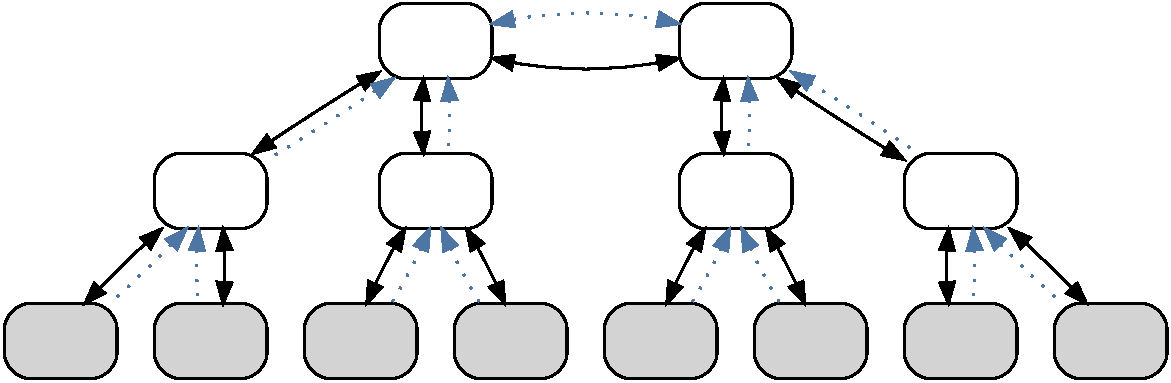
\includegraphics[width=0.2\textwidth]{resources/images/example3}
\end{wrapfigure}

\sidenote{Contributions}
\todomid{write}

\begin{figure}
    \centering
    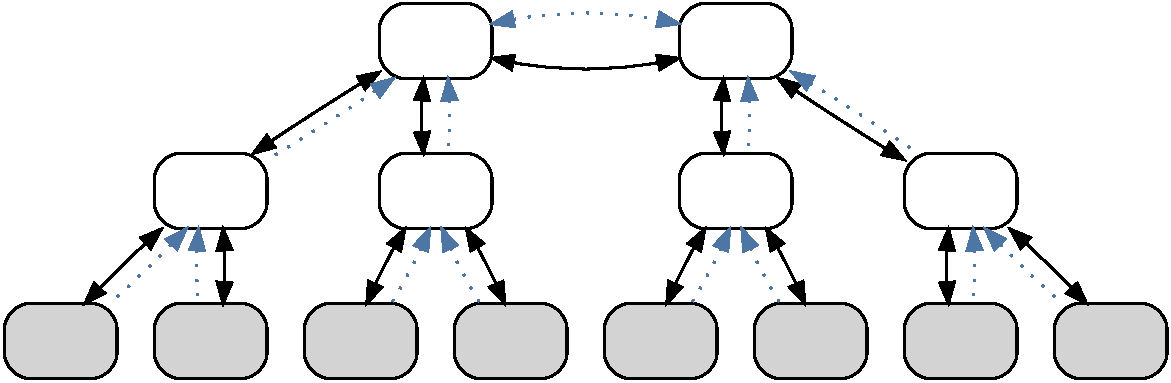
\includegraphics[width=.55\textwidth]{resources/images/example3}
    \caption{Placement of the outlook in the structure of research}\label{fig:hourglass:outlook}
\end{figure}

\sidenote{Dissemination}
\todomid{write about \Cref{fig:hourglass:outlook}}

\section{Conclusions and Impact}

\sidenote{Context}
\todomid{write}

\sidenote{Contribution 1}
\todomid{write}

\sidenote{Contribution 2}
\todomid{write}

\sidenote{Contribution 3}
\todomid{write}

\section{Outlook}

\sidenote{Intro}
\todomid{write}

\sidenote{Application Area 1}
\todomid{write about \Cref{fig:outlook:aa1}}

\begin{figure}
    \centering
    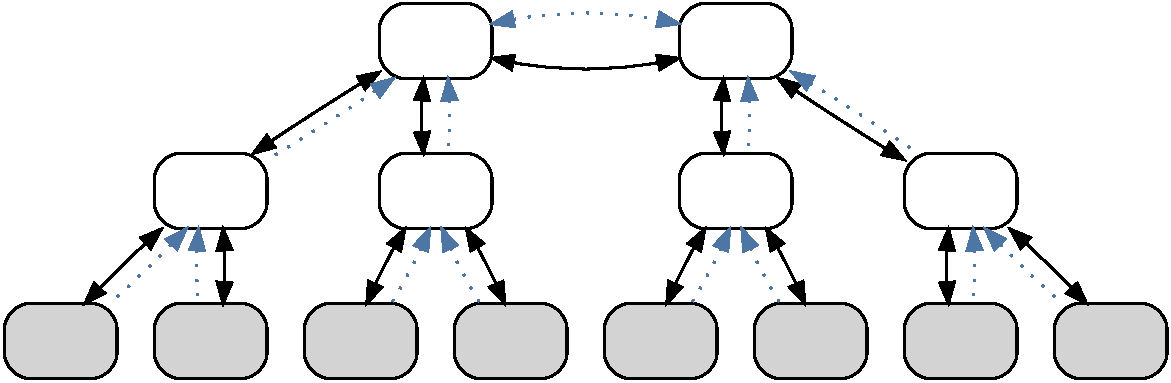
\includegraphics[width=.85\textwidth]{resources/images/example3}
    \caption{Area 1~\cite{li2002design}}\label{fig:outlook:aa1}
\end{figure}

\sidenote{Application Area 2}
\todomid{write}

\sidenote{Application Area 3}
\todomid{write}

\sidenote{Application Area 4}
\todomid{write}

    \nolinenumbers
    \cleardoublepage

    \appendix
    \pagenumbering{Roman}
    \setcounter{page}{1}
    \cleardoublepage\chapter{Specifications}\minitoc\vspace{.5cm}

\section{Specification 1}\index{Specification 1}

\todomid{write about \Cref{lst:spec1}}

\lstset{language=ttl, breaklines=true, caption=Specification 1, %
emptylines=0,
label=lst:spec1, numbers=left, stepnumber=1, inputencoding=utf8}
\lstinputlisting{resources/code/example.java}


\section{Specification 2}\index{Specification 2}

\todomid{write about \Cref{lst:spec2}}

\lstset{language=ttl, breaklines=true, caption=Specification 2, %
emptylines=0,
label=lst:spec2, numbers=left, stepnumber=1, inputencoding=utf8}
\lstinputlisting{resources/code/example.java}


\cleardoublepage\chapter{Test Results}\minitoc\vspace{.5cm}

\section{Conformance Results}

\sidenote{Overview}
\todomid{write about \Cref{fig:test:result1,fig:test:result2}}

\begin{figure}[H]
    \centering
    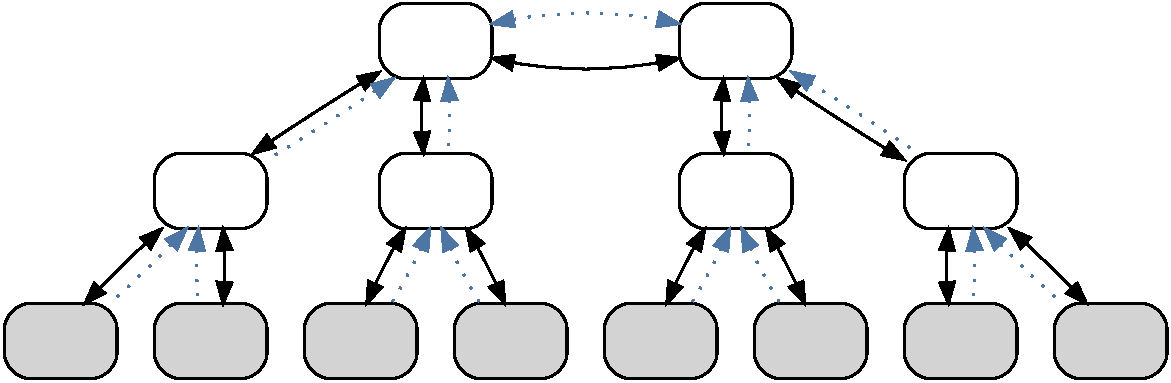
\includegraphics[width=.9\textwidth,frame,page=1]{resources/images/example3}
    \caption{Test results (page 1)}\label{fig:test:result1}
\end{figure}

\begin{figure}[H]
    \centering
    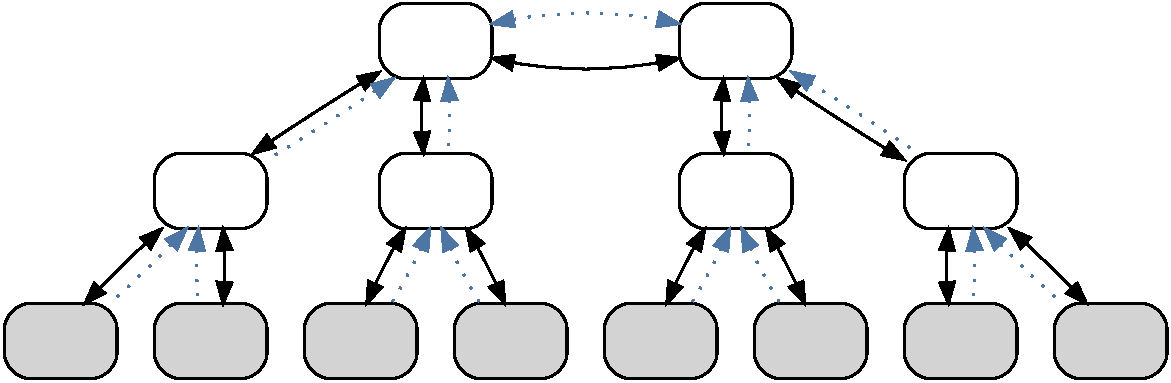
\includegraphics[width=.9\textwidth,frame,page=1]{resources/images/example3}
    \caption{Test results (page 2)}\label{fig:test:result2}
\end{figure}

\section{Performance Results}

\subsection{Histograms}

\sidenote{Overview}
\todomid{write about \Cref{fig:eval:perf:hist:forms}}

\begin{figure}[H]
    \begin{subfigure}[b]{.5\textwidth}
      \centering
      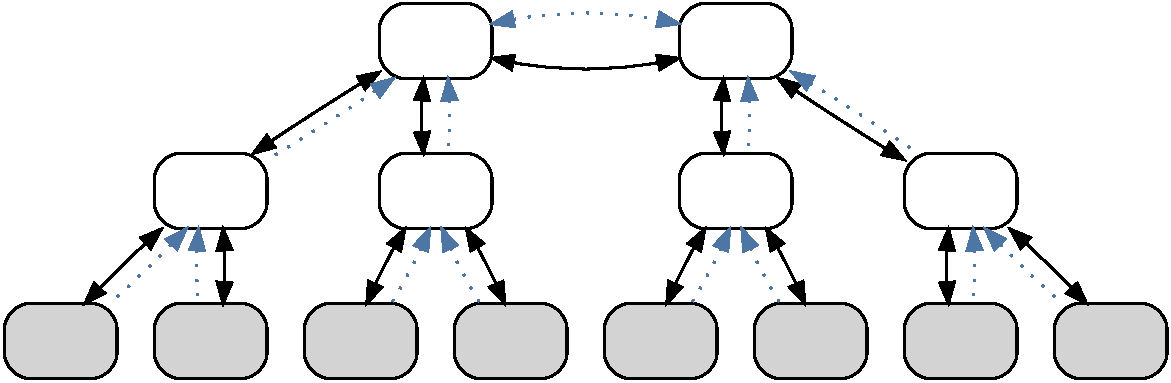
\includegraphics[width=.95\textwidth,frame]{resources/images/example3}
      \caption{Form A}
    \end{subfigure}~\begin{subfigure}[b]{.5\textwidth}
      \centering
      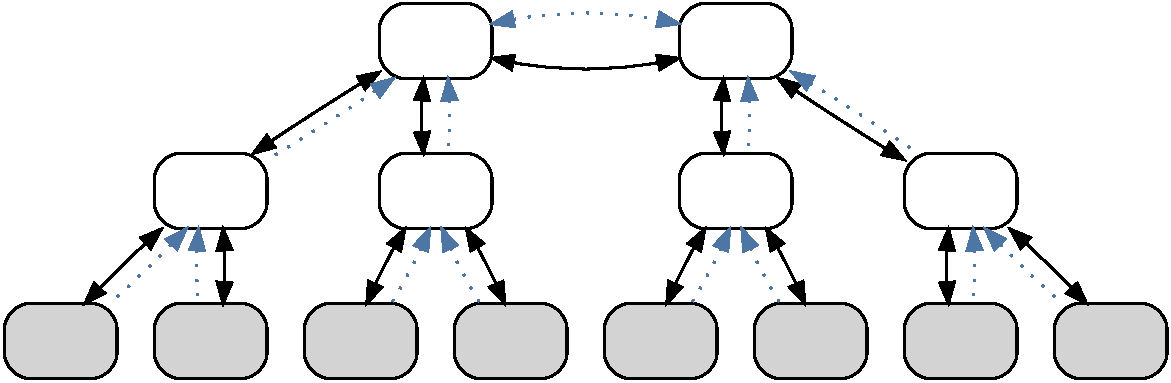
\includegraphics[width=.95\textwidth,frame]{resources/images/example3}
      \caption{Form B}
    \end{subfigure}
    \caption{Histogram of Forms}\label{fig:eval:perf:hist:forms}
\end{figure}


\subsection{Lineplots}

\sidenote{Overview}
\todomid{write about \Cref{fig:eval:perf:line:lines}}

\begin{figure}[H]
    \begin{subfigure}[b]{.5\textwidth}
      \centering
      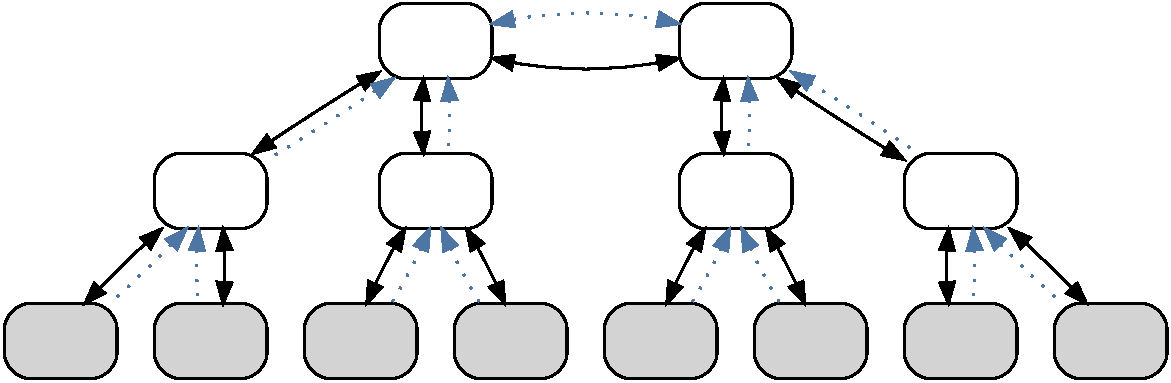
\includegraphics[width=.95\textwidth,frame]{resources/images/example3}
      \caption{Lines A}
    \end{subfigure}~\begin{subfigure}[b]{.5\textwidth}
      \centering
      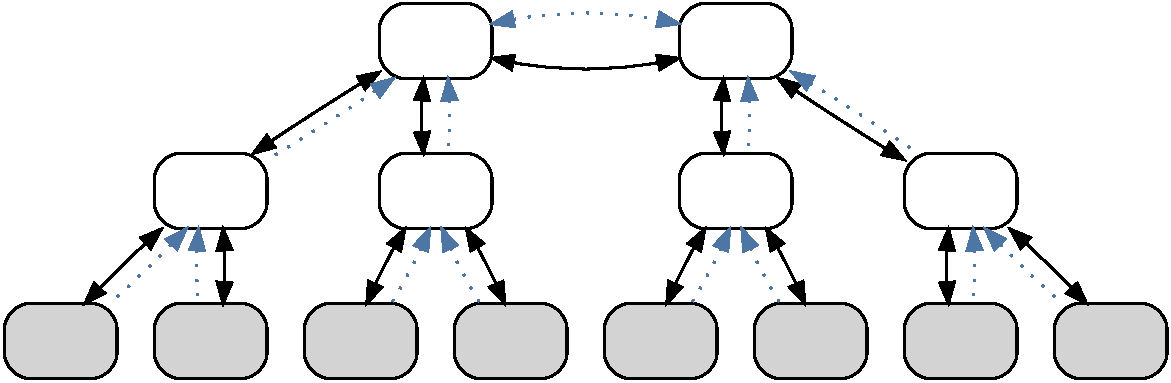
\includegraphics[width=.95\textwidth,frame]{resources/images/example3}
      \caption{Lines A}
    \end{subfigure}
    \caption{Lineplot of the lines}\label{fig:eval:perf:line:lines}
\end{figure}


    \cleardoublepage
    \cleardoublepage
\chapter*{Acronyms}
\mtcaddchapter\addstarredchapter{Acronyms}
\markboth{Acronyms}{Acronyms}
\stepcounter{chapter}
\renewcommand*{\chapterthumbformat}{Acronyms}
\printacronyms[name={}, exclude-classes=exclude]

\cleardoublepage
\stepcounter{chapter}
\renewcommand{\glossaryname}{Glossary}
\markboth{\glossaryname}{\glossaryname}
\renewcommand*{\chapterthumbformat}{\glossaryname}
\printglossary%

\cleardoublepage
\chapter*{Bibliography}
\mtcaddchapter\addstarredchapter{Bibliography}
\markboth{Bibliography}{Bibliography}
\stepcounter{chapter}
\renewcommand*{\chapterthumbformat}{Bibliography}
\minitoc\vspace{.5cm}

\section*{List of Author's Publications Covered in this Thesis}
\nocite{li2002design}
\newrefcontext[labelprefix=a]
\printbibliography[keyword=own,heading=empty,category=cited]


\section*{References to Scientific Publications}
\defbibfilter{papers}{
  type=article
  or type=inproceedings
  or type=proceedings
  or type=journal
  or type=phdthesis
  or type=incollection
  or type=book
  or keyword=thesis
  and not keyword=W3C
  and not keyword=RFC
  and not keyword=ITU
  and not keyword=IEEE
  and not keyword=ANSI
  and not keyword=OGF
  and not keyword=web
  and not keyword=presentation
  and not keyword=workingpaper
}
\newrefcontext[labelprefix=p]
\printbibliography[filter=papers,heading=empty,category=cited,notkeyword=own]


\section*{Technical References}

\defbibfilter{standards}{
  keyword=W3C
  or keyword=RFC
  or keyword=TMF
  or keyword=ITU
  or keyword=IEEE
  or keyword=ANSI
  or keyword=OGF
  or keyword=ETSI
  or keyword=OneM2M
  or keyword=IETF
  or keyword=OMA
  or keyword=TMG
  or keyword=NIST
  or keyword=SNIA
  or keyword=OMG
  or keyword=DMTF
  or keyword=OASIS
  or type=techreport
  or keyword=deliverable
  or keyword=techreport
  or keyword=whitepaper
  and not keyword=web
  and not keyword=presentation
  and not keyword=workingpaper
}
\newrefcontext[labelprefix=t]
\printbibliography[filter=standards,heading=empty,category=cited,notkeyword=own]


\section*{Miscellaneous References}
\defbibfilter{misc}{
  keyword=web
  or keyword=presentation
  or keyword=workingpaper
}
\newrefcontext[labelprefix=m]
\printbibliography[filter=misc,heading=empty,category=cited,notkeyword=own]


\section*{Not referenced (will be empty)}
\todo{this section should be empty at the end}
\nocite{*}
\newrefcontext[labelprefix=x]
\printbibliography[heading=empty,notcategory=cited,notkeyword=own]


    \backmatter
    \cleardoublepage\cleardoublepage
\phantomsection
\stepcounter{chapter}
\renewcommand{\indexname}{Index}
\renewcommand*{\chapterthumbformat}{\indexname}
\markboth{\indexname}{\indexname}
\printindex%

\end{document}
% ------------------------------------------------------------------------------
